\documentclass[11pt,a4paper]{article}
\usepackage[margin=2.3cm]{geometry}
\IfFileExists{lmodern.sty}{\usepackage{lmodern}}{}
\usepackage[T1]{fontenc}
\usepackage{titlesec,tabularx,longtable,booktabs,array,enumitem,xcolor,fancyhdr,amsmath}
\usepackage{listings}
\usepackage{tikz}
\usetikzlibrary{arrows.meta,positioning,fit,calc,shapes.geometric,backgrounds}
\usepackage[hyphens]{url}
\usepackage{hyperref}

\definecolor{headcolor}{RGB}{15,70,60}
\definecolor{boxa}{RGB}{226,239,236}
\definecolor{boxb}{RGB}{238,242,250}
\definecolor{boxc}{RGB}{250,243,230}
\definecolor{boxd}{RGB}{245,245,245}
\definecolor{edge}{RGB}{70,70,70}
\hypersetup{colorlinks=true,linkcolor=headcolor,urlcolor=headcolor,
  pdftitle={TrustBazaar System Design - Unit 1: Identity and Access},
  pdfauthor={S. M. Nihal Ahmed, Afrim Hossen Khan, Sabikun Nahar Sinthia}}

\titleformat{\section}{\normalfont\Large\bfseries\color{headcolor}}{\thesection}{10pt}{}
\titleformat{\subsection}{\normalfont\large\bfseries}{\thesubsection}{8pt}{}
\titleformat{\subsubsection}{\normalfont\normalsize\bfseries}{\thesubsubsection}{6pt}{}
\pagestyle{fancy}\fancyhf{}
\fancyhead[L]{System Design Document}\fancyhead[R]{Unit 1: Identity \& Access}
\fancyfoot[C]{\thepage}\renewcommand{\headrulewidth}{0.4pt}\setlength{\headheight}{14pt}
\setlength{\emergencystretch}{3em}
\setlength{\parskip}{0.45em}\setlength{\parindent}{0pt}

\lstdefinelanguage{SQLpg}{morekeywords={CREATE,TABLE,TYPE,AS,ENUM,PRIMARY,KEY,REFERENCES,NOT,NULL,DEFAULT,CHECK,UNIQUE,INDEX,ON,WHERE,TRIGGER,BEFORE,INSERT,UPDATE,DELETE,FOR,EACH,ROW,EXECUTE,FUNCTION,RETURNS,LANGUAGE,BEGIN,END,IF,THEN,ELSE,RETURN,SELECT,FROM,INTO,ORDER,BY,DESC,LIMIT,GRANT,REVOKE,TO,SCHEMA,EXTENSION,EXISTS,OR,AND,IN,IS,ALTER,ADD,FOREIGN,GENERATED,ALWAYS,IDENTITY,DEFERRABLE,INITIALLY,DEFERRED,DECLARE,PERFORM,LOOP,RAISE,EXCEPTION,USING,DISTINCT,ROLE,LOGIN,USAGE,ALL,TABLES,STABLE,DO},sensitive=false,morecomment=[l]{--},morestring=[b]'}
\lstset{basicstyle=\ttfamily\scriptsize,columns=fullflexible,keepspaces=true,breaklines=true,
  keywordstyle=\color{headcolor}\bfseries,commentstyle=\color{gray}\itshape,frame=single,rulecolor=\color{gray!40},
  upquote=true,literate={–}{{--}}1}

\newenvironment{dtable}[1]{\small\begin{longtable}{#1}}{\end{longtable}}

\begin{document}
\begin{titlepage}
\centering
\vspace*{1cm}
{\Large Daffodil International University}\\[0.2cm]
{\large Department of Software Engineering}\\[2cm]
\rule{\linewidth}{0.5pt}\\[0.4cm]
{\huge\bfseries System Design Document}\\[0.3cm]
{\LARGE Unit 1: Identity \& Access}\\[0.3cm]
{\large TrustBazaar: A Verified Peer-to-Peer Auction and Marketplace Platform for Used Goods}\\[0.2cm]
\rule{\linewidth}{0.5pt}\\[1.6cm]
{\large S. M. Nihal Ahmed (232-35-002)\\[0.1cm] Afrim Hossen Khan (232-35-076)\\[0.1cm] Sabikun Nahar Sinthia (232-35-475)}\\[1.6cm]
\begin{tabular}{|l|>{\raggedright\arraybackslash}p{8cm}|}
\hline
\textbf{Status} & Draft for team review \\ \hline
\textbf{Version} & 0.1, 14 October 2026 \\ \hline
\textbf{Implements} & SRS v2.0 (\texttt{docs/srs.tex}) \\ \hline
\textbf{Database schema} & \texttt{docs/design/sql/01\_identity\_access.sql}, tested on PostgreSQL (46 checks, Appendix B) \\ \hline
\end{tabular}
\vfill
\end{titlepage}
\tableofcontents
\newpage
\section{Introduction}

\subsection{Purpose}
This document is the first unit of TrustBazaar's System Design Document (SDD). It specifies how the \emph{Identity \& Access} unit meets its requirements in the Software Requirements Specification, version 2.0 (``the SRS''). It covers the unit's components, interfaces, database schema, behaviour and security mechanisms. The SDD is being written one unit at a time; when all units are designed, they will be connected into the full system architecture.

This unit is designed first because every other unit depends on it. Every request must answer three questions before anything else happens: who is calling, is that person verified, and what are they allowed to do. This unit also establishes the conventions that all later units follow (Section~\ref{sec:conventions}), and owns two shared mechanisms: the audit log and four-eyes approvals.

\subsection{Planned order of units}
\begin{enumerate}[nosep]
  \item \textbf{Identity \& Access} (this document).
  \item Order, Payment \& Escrow.
  \item Auction Engine; Listings, Search \& Fixed-Price Purchase (in parallel).
  \item Delivery \& Handover.
  \item Game-Account Escrow.
  \item Chat \& Notifications.
  \item Disputes, Trust \& Safety, and Staff Tools.
  \item Frontend: application structure, routing, API client and the screens of every unit, built on the APIs designed above.
  \item Integration: full system architecture, combined data model and deployment view.
\end{enumerate}

\subsection{Scope of this unit}
\textbf{In scope:} registration and phone/e-mail verification; sign-in, MFA, sessions and refresh; step-up authentication; password reset; contact changes; profile and consent records; account closure and erasure; KYC submission, review and revocation; the NID blacklist; staff accounts; four-eyes approvals; the audit log; and the request-authentication and authorisation guards used by every endpoint in the system.

\textbf{Out of scope, owned by later units:} delivering SMS and e-mail (Notifications unit; this unit calls a port, Section~\ref{sec:ports-req}); deciding sanctions (Trust \& Safety unit, which calls this unit's commands to suspend an account or blacklist an identity); parameter versioning and the administrator's parameter screens (Staff Tools unit); and Pro Seller status (Monetization, in the Order unit).

\subsection{Requirements covered}
The unit implements the requirements below; Appendix~\ref{app:trace} maps each one to the design element that satisfies it.
\begin{itemize}[nosep]
  \item \textbf{Functional:} FR-ACC-01 to FR-ACC-11; FR-KYC-01 to FR-KYC-12; FR-TNS-06; FR-OPS-03 to FR-OPS-07 (staff accounts, four-eyes approval, conflicts, staff action logging); FR-PRV-01, FR-PRV-02, FR-PRV-04, FR-PRV-05; FR-NTF-06 (as event source).
  \item \textbf{Security:} SEC-AUTH-01 to SEC-AUTH-12; SEC-SES-01 to SEC-SES-07; SEC-ACC-01 to SEC-ACC-06; SEC-DAT-01 to SEC-DAT-09 and SEC-DAT-11; SEC-INP-04 (KYC uploads); SEC-ABU-01, SEC-ABU-03 (authentication limits); SEC-LOG-01 to SEC-LOG-05.
  \item \textbf{Other:} IF-UI-01, IF-UI-02, IF-UI-09 (staff views); IF-SW-05, IF-SW-06; NFR-USE-02; DR-01, DR-02, DR-09, DR-10.
\end{itemize}

% ------------------------------------------------------------------
\section{Design Conventions for All Units}
\label{sec:conventions}
These conventions are set here because this is the first unit; every later unit follows them unless its own design document records a justified exception.

\begin{dtable}{@{}>{\bfseries}p{1.1cm}>{\raggedright\arraybackslash}p{3.4cm}>{\raggedright\arraybackslash}p{10.6cm}@{}}
\toprule
\textnormal{\textbf{ID}} & \textbf{Convention} & \textbf{Rule} \\ \midrule \endhead
DC-1 & Modular monolith & One NestJS backend (constraint C-1). Each unit is a group of NestJS modules. Units interact only through exported service interfaces (\emph{ports}) and domain events, never by reading another unit's tables or importing its repositories. This keeps the four-container deployment (NFR-MNT-01) while allowing each unit to be designed, tested and later extracted on its own. \\
DC-2 & Layers & Controller (HTTP or WebSocket, request validation) $\rightarrow$ application service (one method per use case, owns the database transaction) $\rightarrow$ repository (TypeORM). Business rules live in services and entities, not in controllers. \\
DC-3 & HTTP API & JSON under \texttt{/api/v1}. Errors use RFC 9457 \texttt{application/problem+json} with a stable \texttt{type}, a user-safe \texttt{title} and the request's \texttt{correlationId} (SEC-INP-06). Lists use cursor pagination. Request bodies are validated by \texttt{class-validator} with \texttt{whitelist} and \texttt{forbidNonWhitelisted} on, so unknown fields are rejected (SEC-INP-01, SEC-ACC-04). \\
DC-4 & Database & One PostgreSQL database, one schema per unit (this unit: \texttt{identity} and \texttt{audit}). Primary keys are random UUIDs (SEC-DAT-11). All times are \texttt{timestamptz}. Money is \texttt{bigint} poisha. Invariants that must never break are enforced by database constraints or triggers as well as in code. Schema changes are versioned migrations; TypeORM \texttt{synchronize} is used only on a developer's machine (NFR-MNT-04). \\
DC-5 & Cross-unit references & A unit may hold a foreign key only to a unit designed \emph{earlier} (in practice, to \texttt{identity.users} and \texttt{identity.staff\_accounts}). References in the other direction are stored as plain UUIDs without a foreign key (for example \texttt{nid\_blacklist.related\_order\_id}). This prevents cycles and keeps each schema loadable on its own. \\
DC-6 & Events & Domain events are named \texttt{<unit>.<entity>.<past\_tense>}. Events whose loss would break a requirement (security notices, KYC decisions, money movements) are written to the unit's \emph{outbox} table in the same transaction as the change, and a background worker publishes them at least once. Consumers must therefore be idempotent. Other events may be emitted in-process after commit. \\
DC-7 & Authorisation & A global guard denies every request by default. Each controller method declares its policy with a decorator (Section~\ref{sec:guards}). A method with no policy cannot be reached. \\
DC-8 & Audit & Every consequential action calls \texttt{AuditService.record()} inside the same database transaction, so the action and its audit entry commit or fail together (SEC-LOG-01). \\
DC-9 & Configuration & Parameters (CP-nn) are read through a \texttt{ConfigPort}, never hard-coded (NFR-MNT-06). Secrets and keys come from environment variables and carry a version number (SEC-DAT-05). \\
DC-10 & Time & Only the server clock is trusted (AS-2). Services receive an injected \texttt{Clock}, so deadlines can be tested without waiting. \\
DC-11 & Shared security middleware & Security headers (\texttt{helmet}: HSTS, CSP with nonces, \texttt{nosniff}, \texttt{Referrer-Policy}, \texttt{Permissions-Policy}), CORS allow-list and cookie parsing are configured once in \texttt{main.ts} as part of this unit (SEC-WEB-01 to SEC-WEB-03). \\
DC-12 & Testing & Each unit has unit tests for its services, integration tests against real PostgreSQL and Redis (the CI service containers), negative authorisation tests for each endpoint (SEC-SDL-09) and, where the database enforces a rule, an SQL test script (Appendix~B). \\
\bottomrule
\end{dtable}

% ------------------------------------------------------------------
\section{Unit Overview}

\subsection{Responsibilities}
\begin{enumerate}[nosep]
  \item Create accounts only for people who have proven control of a Bangladeshi mobile number, and verify their e-mail.
  \item Authenticate users and staff, issue and revoke sessions, and authenticate every HTTP and WebSocket request.
  \item Verify identity through KYC, and guarantee that one NID belongs to at most one account.
  \item Decide, for every request in the system, whether the caller may perform it (roles, KYC status, account status, step-up).
  \item Keep the tamper-evident audit log and run four-eyes approvals for every unit.
  \item Protect identity data: encrypt it, limit and log access to it, and erase it on schedule.
\end{enumerate}

\subsection{Components}
Figure~\ref{fig:components} shows the unit's components. The backend modules map to folders in \texttt{backend/src}: the existing \texttt{auth}, \texttt{users} and \texttt{kyc} modules, plus three new ones, \texttt{staff}, \texttt{audit} and \texttt{security}. The \texttt{security} module is shared infrastructure (guards, cryptography, rate limiting) that every other unit imports.

\begin{figure}[!htbp]
\centering
\resizebox{\textwidth}{!}{%
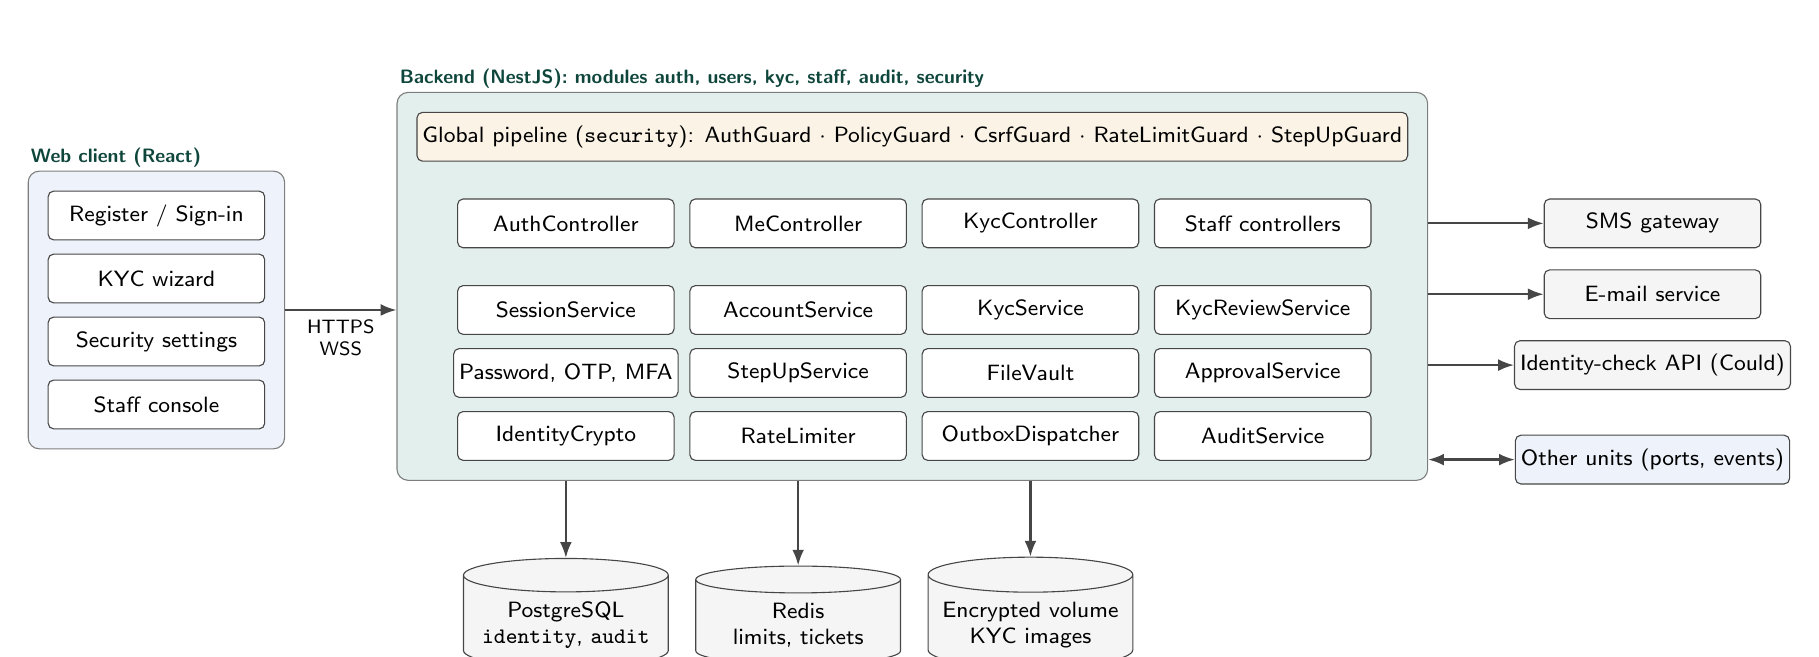
\begin{tikzpicture}[
  font=\sffamily\footnotesize,
  comp/.style={draw=edge, rounded corners=2pt, fill=white, minimum width=2.75cm, minimum height=0.62cm, align=center, inner sep=2pt},
  grp/.style={draw=edge!70, rounded corners=4pt, inner sep=7pt},
  lbl/.style={font=\sffamily\scriptsize\bfseries, text=headcolor, anchor=south west, inner sep=1pt},
  arr/.style={-{Latex[length=2mm]}, draw=edge, thick},
  store/.style={draw=edge, fill=boxd, cylinder, shape border rotate=90, aspect=0.18, minimum width=2.6cm, minimum height=1.1cm, align=center}
]
% client
\node[comp] (c1) at (0,4.0) {Register / Sign-in};
\node[comp] (c2) at (0,3.2) {KYC wizard};
\node[comp] (c3) at (0,2.4) {Security settings};
\node[comp] (c4) at (0,1.6) {Staff console};
\begin{scope}[on background layer]
\node[grp, fill=boxb, fit=(c1)(c4)] (client) {};
\end{scope}
\node[lbl] at (client.north west) {Web client (React)};
% backend
\node[comp, minimum width=11.6cm, fill=boxc] (guards) at (9.6,5.0) {Global pipeline (\texttt{security}): AuthGuard $\cdot$ PolicyGuard $\cdot$ CsrfGuard $\cdot$ RateLimitGuard $\cdot$ StepUpGuard};
\foreach \n/\x/\y/\t in {k1/5.2/3.9/AuthController, k2/8.15/3.9/MeController, k3/11.1/3.9/KycController, k4/14.05/3.9/Staff controllers,
  s1/5.2/2.8/SessionService, s2/8.15/2.8/AccountService, s3/11.1/2.8/KycService, s4/14.05/2.8/KycReviewService,
  s5/5.2/2.0/{Password, OTP, MFA}, s6/8.15/2.0/StepUpService, s7/11.1/2.0/FileVault, s8/14.05/2.0/ApprovalService,
  s9/5.2/1.2/IdentityCrypto, s10/8.15/1.2/RateLimiter, s11/11.1/1.2/OutboxDispatcher, s12/14.05/1.2/AuditService}
  {\node[comp] (\n) at (\x,\y) {\t};}
\begin{scope}[on background layer]
\node[grp, fill=boxa, fit=(guards)(k1)(k4)(s9)(s12)] (be) {};
\end{scope}
\node[lbl] at (be.north west) {Backend (NestJS): modules auth, users, kyc, staff, audit, security};
% stores
\node[store] (pg) at (5.2,-1.2) {PostgreSQL\\\texttt{identity}, \texttt{audit}};
\node[store] (rd) at (8.15,-1.2) {Redis\\limits, tickets};
\node[store] (vol) at (11.1,-1.2) {Encrypted volume\\KYC images};
% external
\node[comp, fill=boxd] (sms) at (19.0,3.9) {SMS gateway};
\node[comp, fill=boxd] (mail) at (19.0,3.0) {E-mail service};
\node[comp, fill=boxd] (idc) at (19.0,2.1) {Identity-check API (Could)};
\node[comp, fill=boxb] (oth) at (19.0,0.9) {Other units (ports, events)};
\draw[arr] (client.east) -- node[below, font=\sffamily\scriptsize, align=center]{HTTPS\\WSS} (be.west|-client.east);
\draw[arr] (pg.north|-be.south) -- (pg.north);
\draw[arr] (rd.north|-be.south) -- (rd.north);
\draw[arr] (vol.north|-be.south) -- (vol.north);
\draw[arr] (be.east|-sms) -- (sms.west);
\draw[arr] (be.east|-mail) -- (mail.west);
\draw[arr] (be.east|-idc) -- (idc.west);
\draw[arr, {Latex[length=2mm]}-{Latex[length=2mm]}] (be.east|-oth) -- (oth.west);
\end{tikzpicture}}
\caption{Components of the Identity \& Access unit. SMS and e-mail are reached through the Notification port; in the academic deliverable they are logged test adapters (AS-4).}
\label{fig:components}
\end{figure}

\begin{dtable}{@{}>{\raggedright\arraybackslash}p{3.2cm}>{\raggedright\arraybackslash}p{12cm}@{}}
\toprule
\textbf{Component} & \textbf{Responsibility} \\ \midrule \endhead
AuthController & Registration, sign-in, MFA challenge, refresh, sign-out, sessions, step-up, password reset (Section~\ref{sec:api}). \\
MeController & Profile, contact changes, MFA enrolment, consents, account closure. \\
KycController & Liveness challenge, KYC submission, status, viewing one's own images. \\
Staff controllers & Staff sign-in, KYC review queue and decisions, approvals, blacklist proposals, conflict declarations; administrator staff management and audit-log view. \\
SessionService & Creates sessions, rotates refresh tokens, detects reuse, ends sessions, records devices. \\
AccountService & Pending registrations, account creation, contact changes, closure and erasure. \\
Password / OTP / MFA & Argon2id hashing and policy checks; OTP generation, hashing and verification; TOTP enrolment, verification and recovery codes. \\
StepUpService & Issues and consumes single-use step-up grants bound to a session and an action. \\
KycService & Validates and stores submissions; computes blind indexes; flags duplicates, blacklist matches and age. \\
KycReviewService & Review queue, claiming, decisions, revocation proposals and the identity-claim guarantee. \\
FileVault & Re-encodes, encrypts, stores, serves and erases KYC images; issues signed view links. \\
ApprovalService & Four-eyes proposals and decisions for all units, with a handler registry. \\
IdentityCrypto & Field encryption, blind indexes and key versions. \\
RateLimiter & Shared Redis counters for every limited endpoint in the system. \\
AuditService & Writes and verifies the hash-chained audit log for all units. \\
OutboxDispatcher & Publishes outbox events and retries failures. \\
\bottomrule
\end{dtable}

\subsection{Libraries}
The stack is fixed by constraint C-1. In addition, this unit uses the following established libraries, chosen so that no cryptography or parsing is written by hand (C-4).
\begin{dtable}{@{}>{\ttfamily}p{3.4cm}>{\raggedright\arraybackslash}p{11.8cm}@{}}
\toprule
\textnormal{\textbf{Library}} & \textbf{Use} \\ \midrule \endhead
argon2 & Argon2id password hashing (SEC-AUTH-03). Replaces the \texttt{bcrypt} dependency currently in \texttt{backend/package.json}. \\
otplib & TOTP generation and verification (RFC 6238). \\
libphonenumber-js & Parsing and validating Bangladeshi mobile numbers into E.164 form. \\
sharp & Decoding, metadata stripping and re-encoding of uploaded images (SEC-DAT-08, SEC-INP-04). \\
file-type & Identifying uploads by their content, not their name (SEC-INP-04). \\
helmet, cookie-parser & Security headers and cookie handling (DC-11). \\
Node.js \texttt{crypto} & AES-256-GCM, HMAC-SHA-256, SHA-256 and secure random bytes. \\
\bottomrule
\end{dtable}
\section{Interfaces}

\subsection{Request authentication and policies}
\label{sec:guards}
Every HTTP request and WebSocket connection passes through the same pipeline before it reaches a controller:
\begin{enumerate}[nosep]
  \item \textbf{RateLimitGuard} applies the endpoint's limit (Section~\ref{sec:redis}); exceeding it returns \texttt{429} with \texttt{Retry-After}.
  \item \textbf{AuthGuard} reads the access-token cookie and verifies the JWT, accepting only HS256 and a known key id (SEC-SES-01). It then loads the session row by its id (the \texttt{sid} claim) together with the principal's status, in one indexed query. The request is rejected unless: the session has not ended; it is within its idle and absolute limits; and the user or staff account is active (or suspended, with the restrictions below). A request is never authenticated by the token alone, so ending a session takes effect on the next request (SEC-SES-05). \texttt{last\_seen\_at} is updated at most once a minute.
  \item \textbf{CsrfGuard}, for every state-changing method, checks the \texttt{Origin} header against the allow-list. It also checks that the \texttt{X-CSRF-Token} header equals the CSRF cookie and that both are an HMAC of the session id (a signed double-submit token, SEC-SES-04).
  \item \textbf{PolicyGuard} enforces the method's declared policy (below). A method without a policy is unreachable (DC-7).
  \item \textbf{StepUpGuard}, for methods marked with \texttt{@StepUp}, consumes a step-up grant (Section~\ref{sec:flow-stepup}).
\end{enumerate}

\begin{dtable}{@{}>{\ttfamily}p{4.6cm}>{\raggedright\arraybackslash}p{10.6cm}@{}}
\toprule
\textnormal{\textbf{Policy decorator}} & \textbf{Allows} \\ \midrule \endhead
@Public() & Anyone, including guests (browsing, registration, sign-in). \\
@SignedIn() & Any user with an active or suspended account. \\
@Verified(action) & A user who is \texttt{verified}, has a verified e-mail, an active (not suspended) account and no restriction for \texttt{action}, where \texttt{action} is one of \texttt{list}, \texttt{bid}, \texttt{buy} or \texttt{payout}. This is the server-side gate of FR-KYC-07, used by all transacting units through \texttt{IdentityQuery.assertCanTransact}. \\
@Staff(role) & An active staff account of the given role whose session satisfied MFA. \\
@StepUp(action) & In addition to the above, a fresh step-up grant for \texttt{action}. \\
\bottomrule
\end{dtable}

A suspended user (FR-TNS-05) can still sign in, see their orders and complete paid ones. \texttt{@Verified} refuses every new listing, bid and purchase.

\subsection{HTTP API}
\label{sec:api}
All paths are under \texttt{/api/v1}. ``RL'' names the rate-limit rule of Section~\ref{sec:redis}. Request and response schemas will be generated as OpenAPI from the DTOs (NFR-MNT-05).

{\small
\begin{longtable}{@{}>{\ttfamily\raggedright\arraybackslash}p{1.15cm}>{\ttfamily\raggedright\arraybackslash}p{5.0cm}>{\raggedright\arraybackslash}p{2.6cm}>{\raggedright\arraybackslash}p{1.5cm}>{\raggedright\arraybackslash}p{4.4cm}@{}}
\toprule
\textnormal{\textbf{Method}} & \textnormal{\textbf{Path}} & \textbf{Policy} & \textbf{RL} & \textbf{Purpose (requirement)} \\ \midrule \endhead
\multicolumn{5}{@{}l}{\textbf{Registration and sign-in}} \\
POST & /\allowbreak auth/\allowbreak register & Public & register & Start registration; send OTP (FR-ACC-01, 03, 04) \\
POST & /\allowbreak auth/\allowbreak register/\allowbreak verify & Public & otp-verify & Verify OTP; create account (FR-ACC-02) \\
POST & /\allowbreak auth/\allowbreak register/\allowbreak resend & Public & otp-send & Resend OTP (SEC-AUTH-09) \\
POST & /\allowbreak auth/\allowbreak email/\allowbreak verify & Public & token & Verify e-mail link (FR-ACC-02) \\
POST & /\allowbreak auth/\allowbreak signin & Public & signin & Password step (FR-ACC-05) \\
POST & /\allowbreak auth/\allowbreak signin/\allowbreak mfa & MFA ticket & otp-verify & Second factor (FR-ACC-06) \\
POST & /\allowbreak auth/\allowbreak refresh & Refresh cookie & refresh & Rotate tokens (SEC-SES-02) \\
POST & /\allowbreak auth/\allowbreak signout & SignedIn & --- & End this session (SEC-SES-05) \\
\multicolumn{5}{@{}l}{\textbf{Sessions, step-up and passwords}} \\
GET & /\allowbreak auth/\allowbreak sessions & SignedIn & --- & List sessions (FR-ACC-08) \\
DELETE & /\allowbreak auth/\allowbreak sessions/\allowbreak \{id\} & SignedIn & --- & End one session \\
POST & /\allowbreak auth/\allowbreak sessions/\allowbreak end-others & SignedIn & --- & End all other sessions \\
POST & /\allowbreak auth/\allowbreak step-up/\allowbreak start & SignedIn & otp-send & Begin step-up for an action \\
POST & /\allowbreak auth/\allowbreak step-up/\allowbreak verify & SignedIn & otp-verify & Obtain a step-up grant (SEC-AUTH-08) \\
POST & /\allowbreak auth/\allowbreak password/\allowbreak forgot & Public & reset & Send reset link or OTP (FR-ACC-07) \\
POST & /\allowbreak auth/\allowbreak password/\allowbreak reset & Public & token & Set new password (SEC-AUTH-10) \\
POST & /\allowbreak auth/\allowbreak password/\allowbreak change & StepUp & --- & Change password (SEC-AUTH-11) \\
\multicolumn{5}{@{}l}{\textbf{Profile, contacts, MFA, consent, closure}} \\
GET & /\allowbreak me & SignedIn & --- & Own account \\
PATCH & /\allowbreak me & SignedIn & --- & Display name, area (FR-ACC-10) \\
GET & /\allowbreak users/\allowbreak \{id\}/\allowbreak profile & Public & search & Public profile (FR-ACC-10) \\
POST & /\allowbreak me/\allowbreak phone/\allowbreak change & StepUp & otp-send & OTP to new number (FR-ACC-09) \\
POST & /\allowbreak me/\allowbreak phone/\allowbreak change/\allowbreak verify & SignedIn & otp-verify & Confirm new number \\
POST & /\allowbreak me/\allowbreak email/\allowbreak change & StepUp & token & Link to new e-mail (FR-ACC-09) \\
POST & /\allowbreak me/\allowbreak mfa/\allowbreak totp & SignedIn & --- & Start TOTP enrolment (FR-ACC-06) \\
POST & /\allowbreak me/\allowbreak mfa/\allowbreak totp/\allowbreak confirm & SignedIn & otp-verify & Confirm; issue recovery codes \\
DELETE & /\allowbreak me/\allowbreak mfa/\allowbreak totp & StepUp & --- & Turn MFA off \\
POST & /\allowbreak me/\allowbreak mfa/\allowbreak recovery-codes & StepUp & --- & Regenerate recovery codes \\
GET, POST & /\allowbreak me/\allowbreak consents & SignedIn & --- & Optional consents (FR-PRV-02) \\
POST & /\allowbreak me/\allowbreak close & StepUp & --- & Close account (FR-ACC-11) \\
\multicolumn{5}{@{}l}{\textbf{KYC (user)}} \\
GET & /\allowbreak kyc/\allowbreak status & SignedIn & --- & Status and reason (IF-UI-02) \\
GET & /\allowbreak kyc/\allowbreak liveness-challenge & SignedIn & kyc & Random action (FR-KYC-02) \\
POST & /\allowbreak kyc/\allowbreak submissions & SignedIn & kyc & Submit documents (FR-KYC-01) \\
POST & /\allowbreak kyc/\allowbreak files/\allowbreak \{kind\}/\allowbreak view & SignedIn & --- & Signed link to own image \\
GET & /\allowbreak files/\allowbreak v/\allowbreak \{token\} & Signed link & files & Stream a protected image (SEC-DAT-04) \\
\multicolumn{5}{@{}l}{\textbf{Staff: operators}} \\
POST & /\allowbreak staff/\allowbreak auth/\allowbreak signin, /\allowbreak staff/\allowbreak auth/\allowbreak mfa & Public & signin & Staff sign-in (SEC-AUTH-07) \\
POST & /\allowbreak staff/\allowbreak auth/\allowbreak mfa/\allowbreak enrol & Pending staff & --- & First MFA enrolment \\
GET & /\allowbreak staff/\allowbreak kyc/\allowbreak queue & Staff(operator) & --- & Oldest first, with flags (FR-OPS-01) \\
POST & /\allowbreak staff/\allowbreak kyc/\allowbreak submissions/\allowbreak \{id\}/\allowbreak claim & Staff(operator) & --- & Take for review (SEC-ACC-06) \\
GET & /\allowbreak staff/\allowbreak kyc/\allowbreak submissions/\allowbreak \{id\} & Staff(operator) & --- & Details (claimant only) \\
POST & /\allowbreak staff/\allowbreak kyc/\allowbreak submissions/\allowbreak \{id\}/\allowbreak files/\allowbreak \{kind\}/\allowbreak view & Staff(operator) & files & Signed link, reason required \\
POST & /\allowbreak staff/\allowbreak kyc/\allowbreak submissions/\allowbreak \{id\}/\allowbreak decision & Staff(operator) & --- & Approve or reject (FR-KYC-06) \\
POST & /\allowbreak staff/\allowbreak users/\allowbreak \{id\}/\allowbreak kyc/\allowbreak revoke & Staff(operator) & --- & Propose revocation (FR-KYC-10) \\
POST & /\allowbreak staff/\allowbreak blacklist & Staff(operator) & --- & Propose blacklisting (FR-TNS-06) \\
POST & /\allowbreak staff/\allowbreak blacklist/\allowbreak \{id\}/\allowbreak remove & Staff(operator) & --- & Propose removal \\
GET & /\allowbreak staff/\allowbreak approvals & Staff(any) & --- & Open proposals for my role \\
POST & /\allowbreak staff/\allowbreak approvals/\allowbreak \{id\}/\allowbreak decision & Staff(required role) & --- & Approve or reject (FR-OPS-05) \\
POST & /\allowbreak staff/\allowbreak conflicts & Staff(any) & --- & Declare a conflict (FR-OPS-06) \\
\multicolumn{5}{@{}l}{\textbf{Staff: administrators}} \\
GET, POST & /\allowbreak admin/\allowbreak staff & Staff(admin) & --- & List, create staff (FR-OPS-04) \\
POST & /\allowbreak admin/\allowbreak staff/\allowbreak \{id\}/\allowbreak disable & Staff(admin) & --- & Disable a staff account \\
POST & /\allowbreak admin/\allowbreak staff/\allowbreak \{id\}/\allowbreak mfa-reset & Staff(admin) & --- & Propose MFA reset (four-eyes) \\
GET & /\allowbreak admin/\allowbreak audit, /\allowbreak admin/\allowbreak audit/\allowbreak verify & Staff(admin) & --- & Read and verify the log (SEC-LOG-04) \\
\bottomrule
\end{longtable}
}

The first administrator is created by a command run inside the backend container (\texttt{npm run staff:bootstrap}). The command refuses to run if any administrator already exists, and the database permits only one account without a creator (FR-OPS-04).

\subsection{Ports provided to other units}
\label{sec:ports}
Other units use this unit only through the following interfaces, exported from the \texttt{auth}, \texttt{kyc}, \texttt{staff} and \texttt{audit} modules.

\begin{lstlisting}[language=Java,morekeywords={interface,type,Promise,string,boolean,void,readonly}]
interface IdentityQuery {
  getPrincipal(userId: string): Promise<{ id: string; displayName: string;
      kycStatus: KycStatus; accountStatus: AccountStatus; emailVerified: boolean }>;
  assertCanTransact(userId: string, action: 'list' | 'bid' | 'buy' | 'payout'): Promise<void>; // throws
  getPublicProfile(userId: string): Promise<PublicProfile>;          // FR-ACC-10 fields only
  getVerifiedPhone(userId: string): Promise<string>;                 // payout wallet match, FR-PAY-17
  getKycLegalName(userId: string, purpose: 'bank_payout_check'):     // decrypts; audited
      Promise<string>;
  hasConflict(staffId: string, userId: string): Promise<boolean>;    // FR-OPS-06
}
interface IdentityCommands {               // called by Trust & Safety; each call is audited
  suspendAccount(userId: string, reason: string, byStaffId: string): Promise<void>;  // ends sessions
  reinstateAccount(userId: string, approvalId: string): Promise<void>;
  endAllSessions(userId: string, reason: SessionEndReason): Promise<void>;
  proposeBlacklist(userId: string, source: BlacklistSource, relatedOrderId: string | null,
      reason: string, byStaffId: string): Promise<Approval>;
}
interface ApprovalService {                // four-eyes for every unit (FR-OPS-05)
  propose(p: { action: string; targetType: string; targetId: string; payload: object;
      reason: string; requiredRole: StaffRole; byStaffId: string }): Promise<Approval>;
  decide(id: string, byStaffId: string, decision: 'approved' | 'rejected', note?: string): Promise<void>;
  registerHandler(action: string, h: (a: Approval, tx: EntityManager) => Promise<void>): void;
}
interface AuditService {
  record(e: { actorType: ActorType; actorId?: string; action: string; objectType?: string;
      objectId?: string; before?: object; after?: object; reason?: string; approvalId?: string },
      tx: EntityManager): Promise<void>;     // same transaction as the action (DC-8)
  verifyChain(): Promise<{ intact: boolean; firstBadId?: number }>;
}
interface RateLimiter { consume(rule: string, subject: string): Promise<void> }  // throws 429
\end{lstlisting}

\subsection{Events published}
All events below go through the outbox (DC-6) and carry the user or staff id, the time and a correlation id. The Notifications unit turns the security events into the notices required by FR-NTF-06.
\begin{dtable}{@{}>{\ttfamily}p{6.0cm}>{\raggedright\arraybackslash}p{9.2cm}@{}}
\toprule
\textnormal{\textbf{Event}} & \textbf{Consumers and purpose} \\ \midrule \endhead
identity.user.registered & Notifications (welcome, e-mail verification link). \\
identity.email.verified & None required; available for analytics. \\
identity.signin.new\_device & Notifications: SMS and e-mail alert (FR-NTF-06). \\
identity.password.changed & Notifications: alert (FR-NTF-06). \\
identity.contact.changed & Notifications: alert to the \emph{old} number or e-mail (FR-ACC-09). \\
identity.mfa.enabled, identity.mfa.disabled & Notifications: alert (FR-NTF-06). \\
identity.session.reuse\_detected & Notifications: alert; Trust \& Safety: signal. \\
identity.kyc.submitted & Notifications: confirmation with expected review time (FR-KYC-12). \\
identity.kyc.verified, identity.kyc.rejected & Notifications (FR-NTF-03); Listings may publish drafts. \\
identity.kyc.revoked & Listings: hide active listings; Auctions and Orders: refuse new bids and purchases (FR-KYC-10). \\
identity.account.suspended, identity.account.reinstated & Listings: hide or restore; Notifications (FR-TNS-03, FR-TNS-05). \\
identity.account.closed & All units: stop processing for the user. \\
\bottomrule
\end{dtable}

\subsection{Ports required from other units}
\label{sec:ports-req}
\begin{dtable}{@{}>{\ttfamily}p{4.4cm}>{\raggedright\arraybackslash}p{10.8cm}@{}}
\toprule
\textnormal{\textbf{Port}} & \textbf{Provided by, and use} \\ \midrule \endhead
NotificationPort & Notifications unit. \texttt{sendSms(phone, template, vars)} for OTPs and security alerts; \texttt{sendEmail(address, template, vars)} for links. Until that unit exists, a test adapter writes messages to the log and a development mailbox, labelled as simulated (AS-4). OTPs are sent synchronously through this port rather than through the outbox, because the user is waiting for them. \\
AccountClosureCheck[] & Orders, Auctions, Payments and Disputes units each register a check. A check returns the reasons, if any, why the user cannot close the account yet (open order, unpaid win, open dispute, balance owed), as required by FR-ACC-11. \\
ConfigPort & Staff Tools unit (parameter store); initially environment configuration. Returns CP-nn values. \\
IdentityCheckPort & Optional pre-check provider (FR-KYC-11, Could). Returns advisory scores only. \\
\bottomrule
\end{dtable}
\section{Data Design}
\label{sec:data}
The complete schema is in \texttt{docs/design/sql/01\_identity\_access.sql} and is reproduced in Appendix~\ref{app:ddl}. It has been loaded into PostgreSQL and checked by a test script of 46 cases (Appendix~\ref{app:tests}). This section explains the structure and the rules the database itself enforces.

\subsection{Schemas}
The unit owns two schemas: \texttt{identity} (20 tables) for accounts, credentials, sessions, KYC, staff and approvals, and \texttt{audit} (one table) for the system-wide audit log. Other units will reference \texttt{identity.users(id)} and \texttt{identity.staff\_accounts(id)} by foreign key; this unit references no other unit (DC-5).

\tikzset{
  ent/.style={draw=edge, fill=white, rounded corners=1.5pt, align=left, inner sep=3pt, font=\sffamily\scriptsize, text width=3.55cm},
  fk/.style={-{Latex[length=1.6mm]}, draw=edge!80, semithick},
}
\newcommand{\ent}[2]{\textbf{\color{headcolor}#1}\\[-1pt]{\ttfamily\tiny #2}}

\begin{figure}[!htbp]
\centering
\resizebox{0.98\textwidth}{!}{%
\begin{tikzpicture}
\node[ent, fill=boxa, text width=4.1cm] (users) at (5.2,3.2) {\ent{users}{id PK\\phone\_e164 (unique while open)\\email (unique while open)\\password\_hash (Argon2id)\\password\_single\_factor\_ok\\mfa\_enabled\\kyc\_status, account\_status\\area, approx\_lat/lng\\closed\_at, erase\_after, erased\_at}};
\node[ent] (pend) at (0,6.2) {\ent{pending\_registrations}{id PK\\phone, email, display\_name\\password\_hash, consents\\expires\_at, completed\_at}};
\node[ent] (otp) at (0,3.6) {\ent{otp\_challenges}{id PK\\purpose, phone\_e164\\code\_hash (HMAC)\\attempts $\le$ max\_attempts\\expires\_at, consumed\_at}};
\node[ent] (ott) at (0,1.3) {\ent{one\_time\_tokens}{id PK\\purpose, token\_hash UNIQUE\\new\_email, expires\_at, used\_at}};
\node[ent] (cons) at (0,-0.8) {\ent{consents}{id PK\\document, version, granted\\recorded\_at, source\_ip}};
\node[ent] (dev) at (10.4,6.2) {\ent{known\_devices}{id PK\\device\_key\_hash\\UNIQUE (user\_id, device\_key\_hash)}};
\node[ent] (sess) at (10.4,3.6) {\ent{sessions}{id PK (= sid claim)\\principal\_type, user\_id | staff\_id\\idle / absolute expiry\\ended\_at, end\_reason}};
\node[ent] (rt) at (10.4,0.9) {\ent{refresh\_tokens}{id PK\\token\_hash UNIQUE\\used\_at, replaced\_by\\one live token per session}};
\node[ent] (totp) at (5.2,-0.2) {\ent{totp\_factors}{id PK, user\_id | staff\_id\\secret\_enc, key\_version\\confirmed\_at, last\_used\_step}};
\node[ent] (rec) at (5.2,-2.3) {\ent{recovery\_codes}{id PK\\code\_hash, used\_at}};
\draw[fk] (otp.east) -- (users.west|-otp.east);
\draw[fk] (otp.north) -- (pend.south);
\draw[fk] (ott.east) -- ++(0.6,0) |- ([yshift=-6pt]users.west);
\draw[fk] (cons.east) -- ++(0.9,0) |- ([yshift=-14pt]users.west);
\draw[fk] (dev.west) -| ([xshift=10pt]users.north);
\draw[fk] (sess.west) -- (users.east|-sess.west);
\draw[fk] (sess.north) -- (dev.south);
\draw[fk] (rt.north) -- (sess.south);
\draw[fk] (rt.east) -- ++(0.35,0) |- node[pos=0.25, right, font=\sffamily\tiny]{replaced\_by} ([yshift=-8pt]rt.east);
\draw[fk] (totp.north) -- (users.south);
\draw[fk] (rec.north) -- (totp.south);
\end{tikzpicture}}
\caption{Accounts and authentication tables (schema \texttt{identity}). Arrows point from the referencing table to the referenced one. \texttt{sessions} and \texttt{totp\_factors} also reference \texttt{staff\_accounts} (Figure~\ref{fig:er-kyc}).}
\label{fig:er-auth}
\end{figure}

\begin{figure}[!htbp]
\centering
\resizebox{0.98\textwidth}{!}{%
\begin{tikzpicture}
\node[ent, fill=boxa] (users) at (0,6.0) {\ent{users}{(Figure~\ref{fig:er-auth})}};
\node[ent] (sub) at (0,3.2) {\ent{kyc\_submissions}{id PK, user\_id\\doc\_type, *\_enc fields\\doc\_number\_bidx, person\_bidx\\is\_adult, liveness\_action\\routed\_flags, status\\claimed\_by/until, decided\_by/at\\rejection\_reason, erased\_at}};
\node[ent] (files) at (0,-0.2) {\ent{kyc\_files}{id PK, submission\_id\\kind, storage\_key\\wrapped\_dek, key\_version\\sha256, mime, byte\_size}};
\node[ent, fill=boxc] (claims) at (5.0,3.2) {\ent{identity\_claims}{doc\_number\_bidx PK\\user\_id UNIQUE\\submission\_id}};
\node[ent] (hist) at (5.0,-0.2) {\ent{kyc\_status\_history}{append-only\\from\_status, to\_status\\actor, reason, approval\_id}};
\node[ent] (conf) at (5.0,6.0) {\ent{staff\_conflicts}{(staff\_id, user\_id) PK\\reason, declared\_at}};
\node[ent, fill=boxa] (staff) at (10.0,6.0) {\ent{staff\_accounts}{id PK, email UNIQUE\\role, status\\password\_hash, phone, nid\_bidx\\created\_by (one bootstrap)}};
\node[ent] (appr) at (10.0,3.2) {\ent{approvals}{id PK, action, target\\reason, required\_role\\proposed\_by $\neq$ decided\_by\\decision, executed\_at}};
\node[ent] (bl) at (10.0,-0.2) {\ent{nid\_blacklist}{id PK, doc\_number\_bidx\\(one active per identity)\\source, related\_order\_id\\add / remove approval}};
\node[ent] (wa) at (14.6,6.0) {\ent{webauthn\_credentials}{id PK, staff\_id\\credential\_id UNIQUE\\public\_key, sign\_count}};
\node[ent, fill=boxd] (aud) at (14.6,3.2) {\ent{audit.events}{id, chain\_pos UNIQUE\\actor, action, object\\before / after, reason\\prev\_hash, hash}};
\node[ent, fill=boxd] (ob) at (14.6,0.6) {\ent{outbox}{id, event\_type\\aggregate\_id, payload\\attempts, dispatched\_at}};
\draw[fk] (sub.north) -- (users.south);
\draw[fk] (files.north) -- (sub.south);
\draw[fk] (claims.west) -- (sub.east|-claims.west);
\draw[fk] (claims.north west) -- (users.south east);
\draw[fk] (hist.north west) -- ([yshift=-4pt]sub.south east);
\draw[fk] (hist.east) -- ++(0.75,0) |- ([yshift=-8pt]appr.west);
\draw[fk] (conf.west) -- (users.east|-conf.west);
\draw[fk] (conf.east) -- (staff.west|-conf.east);
\draw[fk] (appr.north) -- (staff.south);
\draw[fk] (bl.north) -- (appr.south);
\draw[fk] ([yshift=-0.95cm]sub.east) -- node[below, pos=0.55, font=\sffamily\tiny]{claimed\_by, decided\_by (to staff\_accounts)} (7.85,2.25) |- ([yshift=8pt]appr.west);
\draw[fk] (wa.west) -- (staff.east|-wa.west);
\end{tikzpicture}}
\caption{KYC, staff, approvals and audit tables. \texttt{identity\_claims} (shaded) is what makes ``one identity, one account'' a database guarantee. \texttt{audit.events} and \texttt{outbox} have no foreign keys, so any unit can write to the audit log.}
\label{fig:er-kyc}
\end{figure}

\subsection{Tables}
\begin{dtable}{@{}>{\ttfamily\raggedright\arraybackslash}p{3.6cm}>{\raggedright\arraybackslash}p{5.2cm}>{\raggedright\arraybackslash}p{6.4cm}@{}}
\toprule
\textnormal{\textbf{Table}} & \textbf{Holds} & \textbf{Rules enforced by the database} \\ \midrule \endhead
users & One row per account; created only after phone OTP. & Mobile number and e-mail unique among accounts that are not closed (case-insensitive e-mail); Bangladeshi mobile format; Argon2id hashes only; a password under 15 characters only while MFA is on; KYC status changes only along permitted edges (trigger); personal fields may be emptied only after erasure of a closed account. \\
pending\_registrations & Registration details until the OTP is verified. & Password must meet the 15-character rule (no MFA yet); age and terms confirmed. \\
otp\_challenges & Hashed OTPs for registration, step-up, phone change and reset. & Attempts never exceed the maximum; registration OTPs belong to a pending registration; other OTPs belong to a user. \\
one\_time\_tokens & Hashed e-mail verification, e-mail change and reset tokens. & Token hash unique; e-mail-change tokens carry the new address. \\
consents & Terms, privacy and optional consents, with version and time. & --- (append in practice; history kept). \\
known\_devices & Devices previously used by a user (hash of a device cookie). & Unique per user and device. \\
sessions & One sign-in on one device, for a user or a staff member. & Exactly one principal; idle expiry $\le$ absolute expiry; an end reason whenever ended. \\
refresh\_tokens & Rotating refresh tokens of a session. & At most one unused token per session; used tokens record their successor. \\
totp\_factors, recovery\_codes & Encrypted TOTP secrets; hashed recovery codes. & One active factor per principal. \\
webauthn\_credentials & Optional staff passkeys. & Credential id unique. \\
kyc\_submissions & One row per submission, encrypted document details, review state. & One open submission per user; a rejection needs a reason code; an underage submission cannot be approved; decision fields set together; encrypted fields removable only by erasure. \\
kyc\_files & Encrypted images of a submission. & JPEG, PNG or WebP only; at most 10 MB; one file per kind; an erased file has no key. \\
identity\_claims & The identity that each verified account holds. & Primary key on the blind index and unique user: one NID, one account (FR-KYC-04). \\
kyc\_status\_history & Every KYC status change. & Append-only (trigger and grants). \\
staff\_accounts, staff\_conflicts & Operators and administrators; declared conflicts. & Argon2id only; only one account may lack a creator (the bootstrap administrator). \\
approvals & Four-eyes proposals for all units. & Proposer $\ne$ decider; one open proposal per action and target; execution only after approval. \\
nid\_blacklist & Banned identities (blind index). & One active entry per identity; addition and removal each reference an approval. \\
outbox & Events awaiting publication. & Event names belong to this unit. \\
audit.events & System-wide audit log. & Append-only (trigger and grants); each row hashed with its predecessor; chain order assigned under a lock. \\
\bottomrule
\end{dtable}

\subsection{Why the important rules live in the database}
Four guarantees are enforced by the database as well as by the service code, because a bug or a race in application code must not be able to break them:
\begin{enumerate}[nosep]
  \item \textbf{One identity, one account.} Approving a KYC submission inserts its blind index into \texttt{identity\_claims} in the same transaction. Two operators approving two accounts with the same NID at the same moment cannot both succeed; the second transaction fails on the primary key and is rolled back.
  \item \textbf{Linear refresh rotation.} The partial unique index allows only one unused refresh token per session, so two concurrent refreshes cannot both mint a valid successor. The successor link is checked at commit (a deferrable foreign key), so the old token can be marked used before its successor is inserted.
  \item \textbf{Four-eyes.} The check \texttt{decided\_by <> proposed\_by} makes self-approval impossible even through a faulty endpoint. The checks use \texttt{IS NOT DISTINCT FROM} because a plain comparison with a NULL decision evaluates to NULL, which PostgreSQL treats as passing. The test script caught exactly this mistake in the first draft.
  \item \textbf{Tamper-evident audit.} A trigger computes each entry's hash from the previous entry under an advisory lock. Ids are allocated before the lock is taken, so the chain is ordered by a separate \texttt{chain\_pos} assigned inside it. Verification therefore stays correct under concurrent writers, tested with 8 parallel connections. \texttt{audit.verify\_chain()} returns the first entry whose hash does not match.
\end{enumerate}

\subsection{Redis keys}
\label{sec:redis}
Redis holds only short-lived and reconstructible data (NFR-REL-01). Losing it resets counters and expires pending tickets: users repeat a step, but no account, session or decision is lost. OTP attempt limits remain enforced by \texttt{otp\_challenges.attempts} in PostgreSQL even if Redis counters are lost.
\begin{dtable}{@{}>{\ttfamily\raggedright\arraybackslash}p{4.8cm}>{\raggedright\arraybackslash}p{6.0cm}>{\raggedright\arraybackslash}p{4.4cm}@{}}
\toprule
\textnormal{\textbf{Key}} & \textbf{Value and use} & \textbf{Lifetime} \\ \midrule \endhead
rl:\{rule\}:\{subject\} & Fixed-window counter, updated atomically by a Lua script (SEC-ABU-01, SEC-ABU-03). & Window of the rule. \\
signin:fail:\{account\} & Failed sign-in count and delay-until time (SEC-AUTH-04). & CP-04 window. \\
otp:send:\{phone\}:h, :d & OTP sends per number per hour and per day (CP-05). & 1 hour, 1 day. \\
mfa:ticket:\{hash\} & Principal and device waiting for the second factor. & DV-1 (5 min). \\
stepup:\{sid\}:\{action\} & Hash of a single-use step-up grant, consumed with \texttt{GETDEL}. & DV-2 (5 min). \\
liveness:\{challengeId\} & User and the random action for the selfie. & DV-3 (10 min). \\
\bottomrule
\end{dtable}

\begin{dtable}{@{}>{\ttfamily}p{2.2cm}>{\raggedright\arraybackslash}p{5.2cm}>{\raggedright\arraybackslash}p{7.8cm}@{}}
\toprule
\textnormal{\textbf{Rule}} & \textbf{Applies to} & \textbf{Limit} \\ \midrule \endhead
signin & sign-in (user and staff) & CP-04: 5 failures per account per 15 min, then progressive delay; 50 per source address per 15 min. \\
register & registration & 5 per source address per hour. \\
otp-send & any OTP send & CP-05: 3 per number per hour, 10 per day; 10 per source address per hour. \\
otp-verify & any OTP or TOTP entry & CP-05: 5 attempts per challenge; 20 per account per hour. \\
reset & forgotten password & 3 per account per hour; 10 per source address per hour. \\
token & link-token use & 20 per source address per hour. \\
refresh & token refresh & 60 per session per hour. \\
kyc & KYC challenge and submission & 10 per user per day (resubmission limit CP-34 enforced separately). \\
files & signed image links & 120 per staff member per hour (alert at 60, SEC-LOG-05). \\
search & public profile reads & CP-35: 60 per minute per source address. \\
\bottomrule
\end{dtable}

\subsection{Encryption and keys}
\label{sec:keys}
\paragraph{Fields.} Document number, full name, date of birth and TOTP secrets are encrypted with AES-256-GCM. Each value is stored as one byte of key version, a 12-byte random IV, the ciphertext and the 16-byte tag. The \emph{associated data} is the table, column and row id, so a ciphertext copied into another row or column fails to decrypt.

\paragraph{Blind indexes.} \texttt{doc\_number\_bidx} is HMAC-SHA-256 under a separate key, over the document type and the number reduced to digits. \texttt{person\_bidx} is the same HMAC over the normalised full name (lower case, single spaces, Latin script as printed) and the date of birth. It is a second, \emph{non-blocking} signal (\texttt{possible\_duplicate}), because one person may hold NID numbers in different formats, which the number index alone would treat as different people.

\paragraph{Images.} Each KYC image gets a fresh 256-bit data key and is encrypted with AES-256-GCM (associated data: the file id). The data key is wrapped with the key-encryption key, also AES-256-GCM. Files are written with random names and mode \texttt{0600} to a Docker named volume, \texttt{kyc\_vault}, mounted only into the backend container. This keeps within the four-container limit (NFR-MNT-01). Erasure deletes the file and sets \texttt{wrapped\_dek} to NULL (crypto-shredding). A copy of the file in a volume backup can then no longer be decrypted once the database backups that still contain the wrapped key have also expired.

\begin{dtable}{@{}>{\ttfamily}p{3.3cm}>{\raggedright\arraybackslash}p{6.2cm}>{\raggedright\arraybackslash}p{5.7cm}@{}}
\toprule
\textnormal{\textbf{Secret}} & \textbf{Purpose} & \textbf{Rotation} \\ \midrule \endhead
FIELD\_KEY\_V\{n\} & Field encryption (KYC details, TOTP secrets). & New version for new writes; background re-encryption; old version kept until no row uses it. \\
BIDX\_KEY & Blind indexes (documents, persons, staff NIDs). & Rotation requires recomputing every index from decrypted values in one maintenance job; rotate only on compromise. \\
KYC\_KEK\_V\{n\} & Wraps per-file data keys. & Re-wrap data keys only; files are not re-encrypted. \\
JWT\_KEY\_V\{n\} & HS256 access tokens (\texttt{kid} header). & New key signs immediately; previous key accepted for CP-01. \\
CSRF\_KEY, LINK\_KEY & HMAC for CSRF tokens and signed file links. & Any time; outstanding tokens expire within minutes. \\
OTP\_PEPPER & HMAC of OTPs, so that 6-digit codes cannot be brute-forced from a database copy. & On compromise; pending OTPs become invalid. \\
\bottomrule
\end{dtable}
All secrets are read from environment variables at start-up, are never logged, and the backend refuses to start if any is missing or shorter than 32 bytes (SEC-DAT-05).
\section{Behaviour}
Each flow below is one application-service method running in one database transaction unless stated otherwise. Every flow writes its audit entry inside that transaction (DC-8). ``Outbox'' means an event row is written in the same transaction (DC-6).

\subsection{Registration}
\label{sec:flow-register}
\begin{enumerate}[nosep]
  \item \texttt{POST /auth/register} with mobile number, e-mail, display name, password, the accepted terms and privacy versions, and the age confirmation. The mobile number is parsed to E.164 and must be a Bangladeshi mobile number. The password must have at least 15 characters (no MFA exists yet) and must not be in the blocklist of common, breached and context-specific passwords (SEC-AUTH-01, SEC-AUTH-02). The blocklist is a file bundled with the backend, so no password or hash prefix is sent to any outside service.
  \item The password is hashed with Argon2id and a \texttt{pending\_registrations} row is created.
  \begin{itemize}[nosep]
    \item If the number and e-mail are both new, an OTP challenge is created and the code is sent by SMS.
    \item If the number already belongs to an open account, no code is sent. Instead, that account's owner receives an SMS: ``someone tried to register with your number''.
    \item Either way, the response is identical: \texttt{202} with a registration id and a resend time (SEC-AUTH-05, SEC-AUTH-06).
  \end{itemize}
  \item \texttt{POST /auth/register/verify} with the code. The code is compared in constant time with its HMAC; a failure increments \texttt{attempts}, and the database caps attempts at the maximum. On success, one transaction:
  \begin{itemize}[nosep]
    \item creates the \texttt{users} row and the \texttt{consents} rows;
    \item marks the challenge consumed and the registration completed;
    \item creates an e-mail verification token;
    \item writes \texttt{identity.user.registered} to the outbox;
    \item audits \texttt{account.registered}.
  \end{itemize}
  The user is signed in (Section~\ref{sec:flow-signin}).
  \item If the e-mail turns out to belong to another open account, the unique index rejects the insert. The response is then a generic ``could not create an account with these details; if you already have one, sign in or reset your password'', and that account's owner is notified. Residual risk: someone who controls a real Bangladeshi number can learn whether an e-mail address is registered. This is accepted, because each attempt costs a verified SIM and is rate-limited.
  \item The e-mail link (\texttt{POST /auth/email/verify}) sets \texttt{email\_verified\_at}. It is required before the user's first listing, purchase or payout; this is checked by \texttt{@Verified}.
\end{enumerate}

\subsection{Sign-in, MFA and refresh}
\label{sec:flow-signin}
Figure~\ref{fig:seq-signin} shows sign-in with MFA and the refresh rotation, including reuse detection.

\begin{figure}[!htbp]
\centering
\resizebox{\textwidth}{!}{%
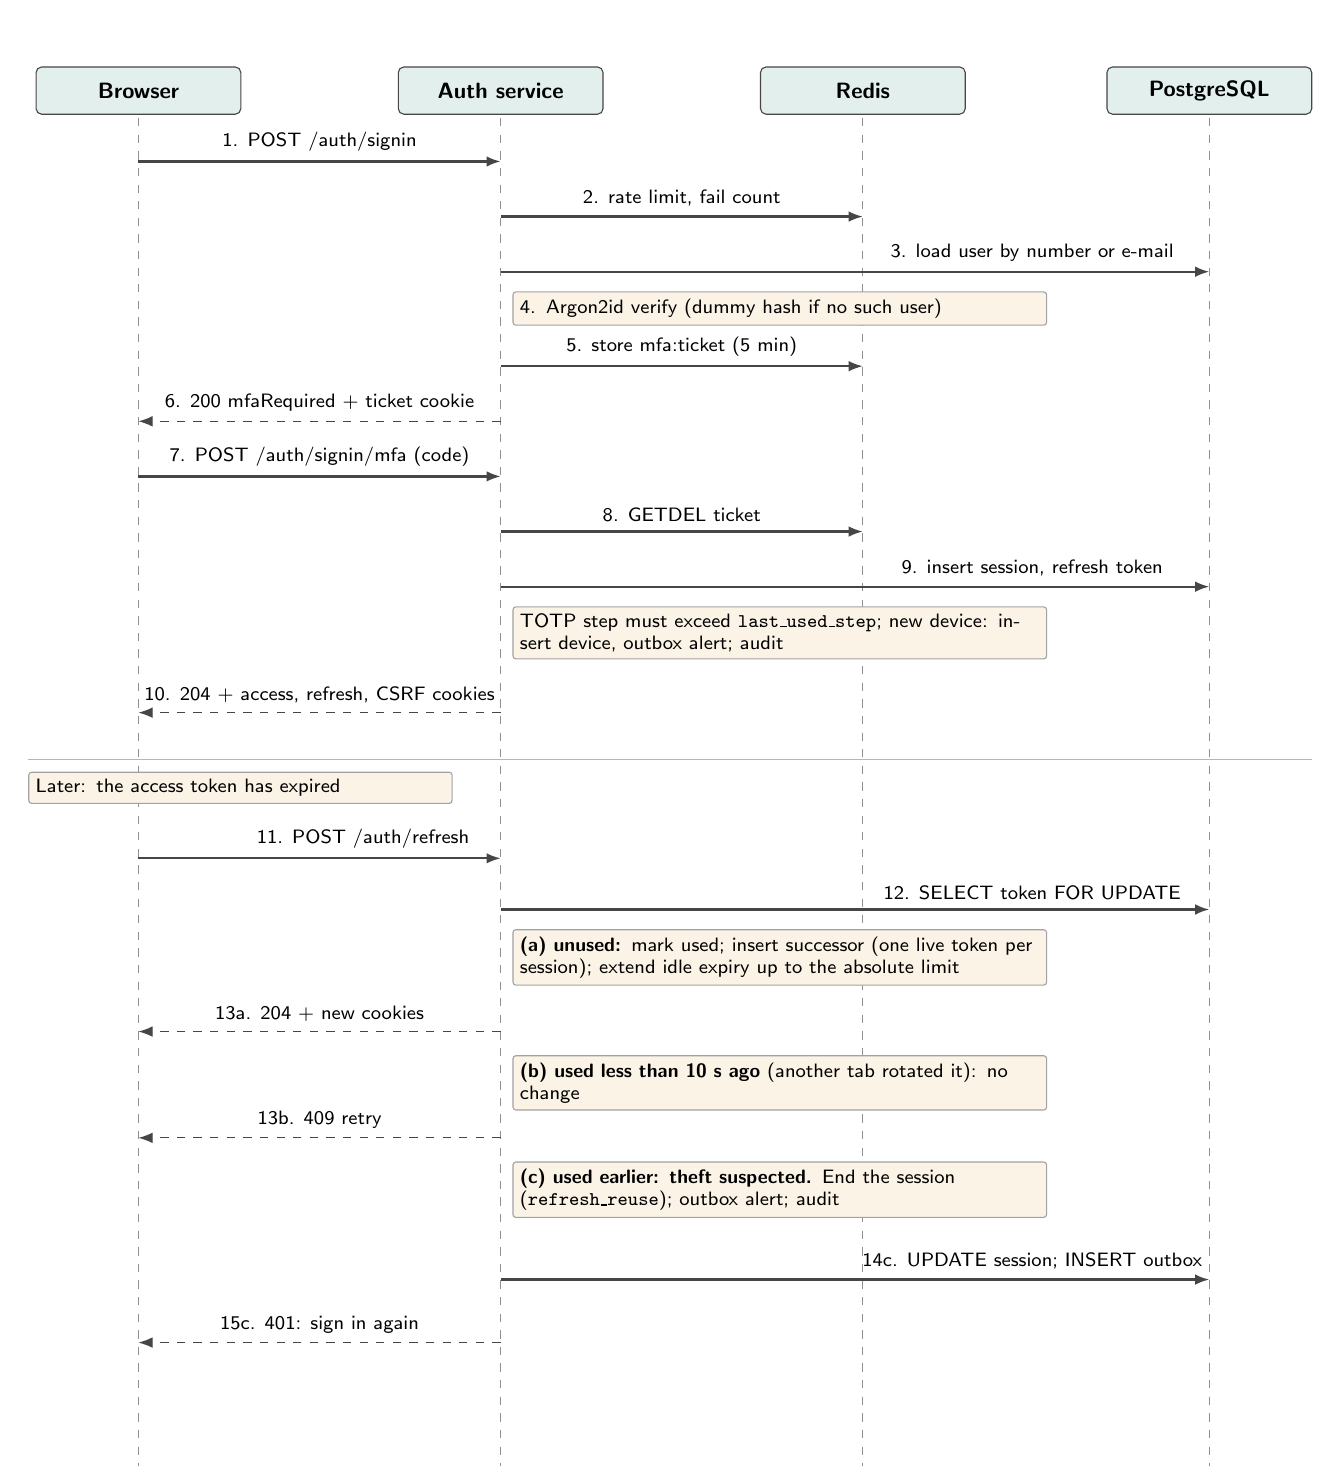
\begin{tikzpicture}[font=\sffamily\scriptsize,
  life/.style={draw=edge!60, dashed},
  hd/.style={draw=edge, fill=boxa, rounded corners=2pt, minimum width=2.6cm, minimum height=0.6cm, font=\sffamily\footnotesize\bfseries},
  msg/.style={-{Latex[length=1.8mm]}, draw=edge, thick},
  ret/.style={-{Latex[length=1.8mm]}, draw=edge, dashed},
  note/.style={draw=edge!50, fill=boxc, align=left, font=\sffamily\scriptsize, inner sep=2.5pt, rounded corners=1pt, text width=6.6cm}]
\def\B{0} \def\A{4.6} \def\R{9.2} \def\P{13.6}
\foreach \x/\n in {\B/Browser, \A/Auth service, \R/Redis, \P/PostgreSQL}{
  \node[hd] at (\x,0) {\n};
  \draw[life] (\x,-0.35) -- (\x,-17.6);}
\draw[msg] (\B,-0.9) -- node[above]{1. POST /auth/signin} (\A,-0.9);
\draw[msg] (\A,-1.6) -- node[above]{2. rate limit, fail count} (\R,-1.6);
\draw[msg] (\A,-2.3) -- node[above, pos=0.75]{3. load user by number or e-mail} (\P,-2.3);
\node[note, anchor=north west] at (\A+0.15,-2.55) {4. Argon2id verify (dummy hash if no such user)};
\draw[msg] (\A,-3.5) -- node[above]{5. store mfa:ticket (5 min)} (\R,-3.5);
\draw[ret] (\A,-4.2) -- node[above]{6. 200 mfaRequired + ticket cookie} (\B,-4.2);
\draw[msg] (\B,-4.9) -- node[above]{7. POST /auth/signin/mfa (code)} (\A,-4.9);
\draw[msg] (\A,-5.6) -- node[above]{8. GETDEL ticket} (\R,-5.6);
\draw[msg] (\A,-6.3) -- node[above, pos=0.75]{9. insert session, refresh token} (\P,-6.3);
\node[note, anchor=north west] at (\A+0.15,-6.55) {TOTP step must exceed \texttt{last\_used\_step}; new device: insert device, outbox alert; audit};
\draw[ret] (\A,-7.9) -- node[above]{10. 204 + access, refresh, CSRF cookies} (\B,-7.9);
\draw[draw=edge!40] (-1.4,-8.5) -- (14.9,-8.5);
\node[note, anchor=north west, text width=5.2cm] at (-1.4,-8.65) {Later: the access token has expired};
\draw[msg] (\B,-9.75) -- node[above, pos=0.62]{11. POST /auth/refresh} (\A,-9.75);
\draw[msg] (\A,-10.4) -- node[above, pos=0.75]{12. SELECT token FOR UPDATE} (\P,-10.4);
\node[note, anchor=north west] at (\A+0.15,-10.65) {\textbf{(a) unused:} mark used; insert successor (one live token per session); extend idle expiry up to the absolute limit};
\draw[ret] (\A,-11.95) -- node[above]{13a. 204 + new cookies} (\B,-11.95);
\node[note, anchor=north west] at (\A+0.15,-12.25) {\textbf{(b) used less than 10 s ago} (another tab rotated it): no change};
\draw[ret] (\A,-13.3) -- node[above]{13b. 409 retry} (\B,-13.3);
\node[note, anchor=north west] at (\A+0.15,-13.6) {\textbf{(c) used earlier: theft suspected.} End the session (\texttt{refresh\_reuse}); outbox alert; audit};
\draw[msg] (\A,-15.1) -- node[above, pos=0.75]{14c. UPDATE session; INSERT outbox} (\P,-15.1);
\draw[ret] (\A,-15.9) -- node[above]{15c. 401: sign in again} (\B,-15.9);
\end{tikzpicture}}
\caption{Sign-in with MFA, and refresh-token rotation with reuse detection (SEC-SES-02). Without MFA, steps 5--8 are skipped and the session is created after step 4.}
\label{fig:seq-signin}
\end{figure}

Further rules:
\begin{itemize}[nosep]
  \item \textbf{Sign-in failure.} Unknown accounts, closed accounts and wrong passwords all receive the same \texttt{401} after the same Argon2id work, so response time does not reveal which accounts exist (SEC-AUTH-05). After \texttt{CP-04} failures, the delay before the next attempt doubles from 1 second up to 15 minutes. A successful password reset always clears the delay, so the owner is never locked out permanently (SEC-AUTH-04). The first delay notifies the owner.
  \item \textbf{TOTP.} Codes are accepted within one 30-second step either side of the current time. The step used is stored, so the same code cannot be used twice. A recovery code may replace the TOTP code once.
  \item \textbf{Hash upgrades.} If the Argon2id parameters stored in a hash are older than the current ones, the password is re-hashed after a successful sign-in.
  \item \textbf{Parallel tabs.} The web client performs refreshes one at a time across tabs, using the browser's Web Locks API, so case (b) of Figure~\ref{fig:seq-signin} is rare. The 10-second grace window (DV-4) covers the rest.
  \item \textbf{Session end.} Sign-out, ``end session'', password change, suspension, closure and staff disablement set \texttt{ended\_at} and \texttt{end\_reason}. The next request with any token of that session fails at AuthGuard. Open WebSocket connections in the room \texttt{sid:\{id\}} are disconnected through the Socket.IO adapter (SEC-SES-05, SEC-SES-07).
\end{itemize}

\subsection{Step-up authentication}
\label{sec:flow-stepup}
\begin{enumerate}[nosep]
  \item \texttt{POST /auth/step-up/start} names one action from a fixed list. The actions are: \texttt{password.change}, \texttt{phone.change}, \texttt{email.change}, \texttt{mfa.disable}, \texttt{recovery.regenerate}, \texttt{payout.change} (used by the Payment unit), \texttt{game.release\_early} (used by the Game-Account unit) and \texttt{account.close}.
  \item If the user has TOTP, no message is sent and the TOTP code is the challenge. Otherwise an OTP with purpose \texttt{step\_up} is sent to the verified number, bound to the session id and the action.
  \item \texttt{POST /auth/step-up/verify} checks the code and returns a single-use grant. Only its hash is kept in Redis, under \texttt{stepup:\{sid\}:\{action\}}, for DV-2.
  \item The sensitive request carries the grant in the \texttt{X-Step-Up} header. StepUpGuard reads and deletes the key atomically (\texttt{GETDEL}) and compares the hash, so a grant works once, for one action, in one session (SEC-AUTH-08).
\end{enumerate}

\subsection{Password reset and change}
\begin{itemize}[nosep]
  \item \texttt{POST /auth/password/forgot} always returns \texttt{202}. If the identifier is a registered e-mail, a 256-bit link token valid for CP-06 is e-mailed. If it is a registered number, a reset OTP is sent by SMS.
  \item \texttt{POST /auth/password/reset} takes the token (or number and OTP) and the new password. \textbf{If the account has MFA enabled, a TOTP or recovery code is also required}, so that access to the e-mail inbox alone cannot remove the second factor. A user who has lost both the authenticator and the recovery codes must re-verify their identity with an operator; that procedure belongs to the Staff Tools unit.
  \item On success, one transaction: sets the new hash and \texttt{password\_single\_factor\_ok}; marks the token used; ends every session with reason \texttt{password\_changed}; writes \texttt{identity.password.changed} to the outbox (SEC-AUTH-10, SEC-AUTH-11).
  \item \texttt{POST /auth/password/change} requires step-up and the current password, and ends every \emph{other} session.
\end{itemize}

\subsection{Contact changes and MFA}
\begin{itemize}[nosep]
  \item \textbf{New number} (FR-ACC-09): step-up, then an OTP to the \emph{new} number; on verification the number is replaced, but only if no other open account holds it (unique index). \texttt{identity.contact.changed} is sent to the \emph{old} number.
  \item \textbf{New e-mail}: step-up, then a link token of purpose \texttt{email\_change} sent to the new address; using it replaces the address and notifies the old one.
  \item \textbf{Enable TOTP}: a 160-bit secret is generated and stored encrypted but unconfirmed, and returned as an \texttt{otpauth://} URI shown as a QR code. Confirming with a valid code sets \texttt{confirmed\_at} and \texttt{users.mfa\_enabled}, and issues ten single-use recovery codes, shown once and stored hashed.
  \item \textbf{Disable TOTP}: step-up plus a current TOTP code. If the password was set under the 8-character MFA rule (\texttt{password\_single\_factor\_ok} is false), the same request must set a new password of at least 15 characters. The database rejects any other outcome (SEC-AUTH-01).
\end{itemize}

\subsection{KYC submission}
\label{sec:flow-kyc}
\begin{enumerate}[nosep]
  \item The user must be in \texttt{unsubmitted} or \texttt{rejected} status and within the resubmission limit CP-34.
  \item \texttt{GET /kyc/liveness-challenge} returns a challenge id and one random action, such as ``turn your head to the left''. The wizard captures two frames through \texttt{getUserMedia}: one neutral, and one while the user performs the action. Gallery files are not accepted (FR-KYC-02).
  \item \texttt{POST /kyc/submissions} (multipart): document type, number, full name, date of birth, the challenge id and four or five images. These are front and back, or passport page, plus the two selfie frames.
  \item Each image is processed in order:
  \begin{enumerate}[nosep]
    \item its type is identified from its content and must be JPEG, PNG or WebP of at most 10 MB;
    \item it is decoded and rotated upright, all metadata including EXIF location is removed, it is resized to at most 2000 pixels on the long side, and it is re-encoded as JPEG;
    \item it is hashed, encrypted with a fresh data key and written to the vault (Section~\ref{sec:keys}).
  \end{enumerate}
  Re-encoding also destroys most payloads hidden in image files. A separate malware scanner would need a fifth container, which NFR-MNT-01 rules out, so SEC-INP-04's ``should scan'' is met by re-encoding, and this is recorded as a deviation in the ASVS checklist (SEC-GEN-01).
  \item The service computes:
  \begin{itemize}[nosep]
    \item \texttt{is\_adult} from the date of birth;
    \item both blind indexes;
    \item the routing flags: \texttt{underage}; \texttt{duplicate} (the document index is claimed by, or pending for, another user); \texttt{possible\_duplicate} (the person index matches another user); \texttt{blacklisted}.
  \end{itemize}
  Flags only route a submission for closer review; they never decide it (FR-KYC-03, FR-KYC-04).
  \item One transaction:
  \begin{itemize}[nosep]
    \item inserts the submission and its file rows;
    \item moves \texttt{kyc\_status} to \texttt{pending\_review};
    \item writes the history row;
    \item audits;
    \item writes \texttt{identity.kyc.submitted} to the outbox.
  \end{itemize}
  The optional pre-check (FR-KYC-11) runs afterwards and may add the \texttt{precheck} flag and its advisory result.
\end{enumerate}
The liveness check is basic, as the SRS states: a user who bypasses the web client can still upload prepared images. Its value is that it makes a reused photograph harder to pass and gives the operator two frames to compare. The operator's review remains the actual control.

\subsection{KYC review, revocation and blacklist}
\label{sec:flow-review}

\begin{figure}[!htbp]
\centering
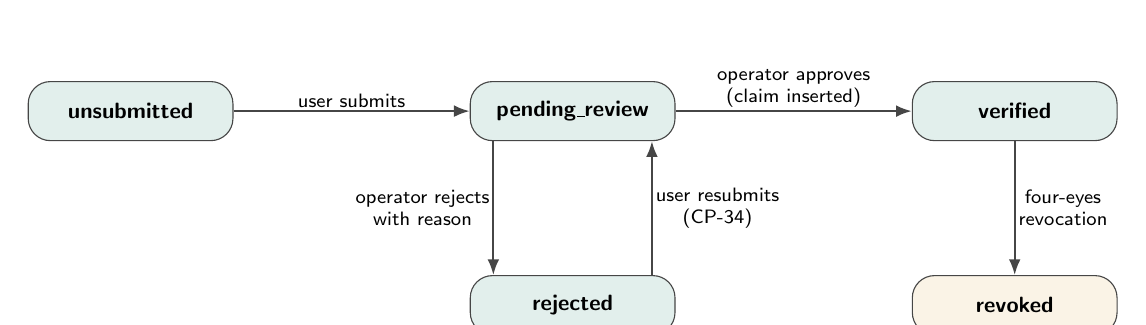
\begin{tikzpicture}[font=\sffamily\footnotesize, node distance=1.2cm and 2.4cm,
  st/.style={draw=edge, rounded corners=8pt, fill=boxa, minimum width=2.6cm, minimum height=0.75cm, font=\sffamily\footnotesize\bfseries},
  tr/.style={-{Latex[length=2mm]}, draw=edge, thick},
  lb/.style={font=\sffamily\scriptsize, align=center, fill=white, inner sep=1pt}]
\node[st] (u) {unsubmitted};
\node[st, right=3.0cm of u] (p) {pending\_review};
\node[st, right=3.0cm of p] (v) {verified};
\node[st, below=1.7cm of p] (r) {rejected};
\node[st, below=1.7cm of v, fill=boxc] (x) {revoked};
\draw[tr] (u) -- node[lb, above]{user submits} (p);
\draw[tr] (p) -- node[lb, above]{operator approves\\(claim inserted)} (v);
\draw[tr] (p.south west) ++(0.3,0) -- node[lb, left]{operator rejects\\with reason} ([xshift=0.3cm]r.north west);
\draw[tr] ([xshift=-0.3cm]r.north east) -- node[lb, right]{user resubmits\\(CP-34)} ([xshift=-0.3cm]p.south east);
\draw[tr] (v) -- node[lb, right]{four-eyes\\revocation} (x);
\end{tikzpicture}
\caption{KYC status of a user (FR-KYC-05). The database trigger \texttt{users\_kyc\_transition} rejects every other change; \texttt{revoked} is final for that account.}
\label{fig:kyc-states}
\end{figure}

\begin{enumerate}[nosep]
  \item \textbf{Queue.} The queue lists pending submissions oldest first, showing their flags and their age against CP-44 (FR-KYC-12).
  \item \textbf{Claim.} An operator claims a submission with a single conditional update: it is assigned only if it is still pending and either unclaimed or its claim has expired (DV-6, 30 minutes). Two operators can therefore never work on the same submission. Claiming is refused if the operator has a conflict with the user: the same mobile number, e-mail or NID blind index as the operator's own, or a declared conflict (FR-OPS-06).
  \item \textbf{Review.} Only the claimant can open the details. Document fields are decrypted for display, and every decryption is audited. Each image is opened through a signed link that requires a reason (Section~\ref{sec:files}).
  \item \textbf{Approve.} One transaction:
  \begin{itemize}[nosep]
    \item locks the submission and re-checks the blacklist;
    \item inserts the \texttt{identity\_claims} row; if another account already holds the identity, the primary key rejects it, and the operator must reject the submission with \texttt{duplicate\_identity};
    \item marks the submission approved and moves the user to \texttt{verified};
    \item writes the history row and the audit entry, and \texttt{identity.kyc.verified} to the outbox.
  \end{itemize}
  \item \textbf{Reject.} A reason code from the fixed list is required, with an optional note shown to the user. The user moves to \texttt{rejected}, and \texttt{identity.kyc.rejected} is written to the outbox (FR-KYC-06).
  \item \textbf{Revoke} (FR-KYC-10). An operator proposes \texttt{kyc.revoke} with a reason. When a second operator approves, the handler moves the user to \texttt{revoked}, records the approval in the history and writes \texttt{identity.kyc.revoked} to the outbox, so that listings are hidden and new bids and purchases refused. The identity claim stays, so the same person cannot verify a new account.
  \item \textbf{Blacklist} (FR-TNS-06, FR-GAM-18). \texttt{blacklist.add} is proposed with the user, the source and the related order. On approval, the handler copies the user's claimed blind index into \texttt{nid\_blacklist}. Removing an entry needs its own approved proposal. Each new KYC submission is checked against active entries.
\end{enumerate}

\subsection{Protected files}
\label{sec:files}
A request to view an image (by the owner, or by the claiming operator with a reason) returns a link \texttt{/api/v1/files/v/\{token\}}. The token is the file id, the requesting session id and an expiry within CP-31, authenticated with HMAC under \texttt{LINK\_KEY}. When the link is used, the server:
\begin{itemize}[nosep]
  \item verifies the HMAC and the expiry;
  \item checks that the request comes from the same session that asked for the link, so a leaked link is useless;
  \item decrypts the file as a stream;
  \item sends it with \texttt{Cache-Control: no-store}, \texttt{X-Content-Type-Options: nosniff}, \texttt{Content-Security-Policy: sandbox} and its fixed image type.
\end{itemize}
Issuing a link to staff is audited as \texttt{kyc.file.viewed} (SEC-ACC-06, SEC-DAT-04). The Disputes unit will issue links to case evidence through the same \texttt{FileVault} port, after its own check that the operator is assigned to the case.

\subsection{Four-eyes approvals}
\label{sec:flow-approvals}
\texttt{ApprovalService.propose()} writes an approval row with the action, target, payload, reason, required role and expiry (DV-5, 72 hours). Staff of the required role see open proposals in their queue. \texttt{decide()} records the decision. If it is ``approved'', the decision also calls the handler registered for that action \emph{in the same transaction} and sets \texttt{executed\_at}. Either the decision and its effect both happen, or neither does. The database prevents self-approval and duplicate open proposals, and a scheduled job marks stale proposals \texttt{expired}. Actions registered by this unit: \texttt{kyc.revoke}, \texttt{blacklist.add}, \texttt{blacklist.remove}, \texttt{account.reinstate} and \texttt{staff.mfa\_reset}. Later units register theirs, for example large dispute outcomes (CP-30).

\subsection{Suspension, closure and erasure}
\begin{itemize}[nosep]
  \item \textbf{Suspension.} The Trust \& Safety unit calls \texttt{IdentityCommands.suspendAccount}. This sets \texttt{account\_status = suspended}, ends all sessions and writes \texttt{identity.account.suspended} to the outbox. The user can sign in again to follow paid orders, but \texttt{@Verified} refuses every new listing, bid and purchase (FR-TNS-05). Reinstatement is the four-eyes action \texttt{account.reinstate}.
  \item \textbf{Closure} (FR-ACC-11). Step-up, then every registered \texttt{AccountClosureCheck} is asked for blocking reasons. If any are returned, the user sees them. Otherwise one transaction:
  \begin{itemize}[nosep]
    \item sets \texttt{closed}, \texttt{closed\_at} and \texttt{erase\_after = closed\_at + CP-41};
    \item ends all sessions;
    \item writes \texttt{identity.account.closed} to the outbox.
  \end{itemize}
  \item \textbf{Erasure} (FR-PRV-04). A daily job processes accounts past \texttt{erase\_after} that no unit holds (the same checks, now asking about legal or dispute holds). It:
  \begin{itemize}[nosep]
    \item replaces the display name with ``Deleted user'' and empties the number, e-mail, password hash and location;
    \item removes MFA factors;
    \item deletes the identity claim;
    \item erases KYC submissions: their encrypted fields and indexes are cleared, image files deleted and data keys destroyed;
    \item sets \texttt{erased\_at}.
  \end{itemize}
  The user row itself remains, because orders and settlements in other units reference it. A blacklist entry keeps its own blind index (SRS Table~7.2). The same job erases KYC data of submissions rejected more than 30 days earlier when the user has not resubmitted.
\end{itemize}

\subsection{Staff accounts}
\begin{itemize}[nosep]
  \item The bootstrap command creates the first administrator in status \texttt{pending\_mfa}. An administrator creates further staff accounts the same way. The initial password is generated, shown once to the creating administrator, and handed over in person.
  \item A staff member in \texttt{pending\_mfa} can only change the password and enrol TOTP or a passkey; then the status becomes \texttt{active} (SEC-AUTH-07).
  \item Disabling a staff account ends its sessions. Resetting a staff member's MFA is the four-eyes action \texttt{staff.mfa\_reset}, which needs a second administrator. With a team of one administrator, it falls back to the bootstrap procedure, which is audited.
  \item Staff sessions use CP-03 limits. Staff accounts cannot reach any \texttt{@Verified} endpoint, because a staff principal is never a user principal (FR-OPS-04).
\end{itemize}
\section{Security Design}

\subsection{Tokens and cookies}
\begin{dtable}{@{}>{\ttfamily\raggedright\arraybackslash}p{2.7cm}>{\raggedright\arraybackslash}p{4.2cm}>{\raggedright\arraybackslash}p{4.8cm}>{\raggedright\arraybackslash}p{3.4cm}@{}}
\toprule
\textnormal{\textbf{Cookie}} & \textbf{Content} & \textbf{Attributes} & \textbf{Lifetime} \\ \midrule \endhead
\_\_Host-tb\_at & Access JWT (HS256, \texttt{kid}; claims \texttt{sub}, \texttt{sid}, \texttt{pt}, \texttt{iat}, \texttt{exp}) & HttpOnly, Secure, SameSite=Strict, Path=/ & CP-01 (15 min) \\
\_\_Secure-tb\_rt & 256-bit random refresh token (server keeps SHA-256) & HttpOnly, Secure, SameSite=Strict, Path=/api/v1/auth/refresh & Session's absolute limit \\
\_\_Host-tb\_csrf & HMAC of the session id (signed double-submit) & Secure, SameSite=Strict, Path=/; \emph{readable} by the client, which copies it into \texttt{X-CSRF-Token} & Same as access token \\
\_\_Host-tb\_mfa & MFA ticket (server keeps hash) & HttpOnly, Secure, SameSite=Strict, Path=/ & DV-1 (5 min) \\
\_\_Host-tb\_dev & 256-bit device key (server keeps hash) & HttpOnly, Secure, SameSite=Strict, Path=/ & 1 year \\
\bottomrule
\end{dtable}
No token is ever placed in \texttt{localStorage}, a URL or a log (SEC-SES-03). The \texttt{\_\_Host-} prefix makes the browser refuse a cookie that is not Secure, has a Domain or has a path other than \texttt{/}, which blocks cookie injection from sibling sub-domains. The refresh cookie uses \texttt{\_\_Secure-} because it is limited to the refresh path, so the refresh token is sent with no other request.

\textbf{Same origin in development and production.} The web client and the API are served from one origin: Vite's development proxy forwards \texttt{/api} to the backend, and in production a reverse proxy does the same. All cookies are therefore first-party, SameSite=Strict works, and CORS is needed only for listed tools (SEC-WEB-03). Browsers treat \texttt{http://localhost} as a secure context, so Secure cookies work in local development; Safari needs the development server's HTTPS option.

\textbf{Changes needed in the repository.} \texttt{frontend/src/api/client.ts} must stop reading a token from \texttt{localStorage}, send requests with \texttt{credentials: 'include'}, and add the \texttt{X-CSRF-Token} header. \texttt{bcrypt} is replaced by \texttt{argon2}. The current \texttt{User} and \texttt{KycDocument} entities in \texttt{backend/src/entities} are replaced by entities matching this schema; their status values (\texttt{unverified}, \texttt{pending}, \texttt{approved}) do not match the SRS, and the single \texttt{role} column mixes Pro Seller with staff roles, which this design separates.

\subsection{Threats and how the design answers them}
\begin{dtable}{@{}>{\raggedright\arraybackslash}p{4.0cm}>{\raggedright\arraybackslash}p{11.2cm}@{}}
\toprule
\textbf{Threat} & \textbf{Design response} \\ \midrule \endhead
Credential stuffing & Per-account progressive delay and per-address limits; breached-password blocklist; MFA option; new-device alerts (SEC-AUTH-02, SEC-AUTH-04, SEC-AUTH-12). \\
Account enumeration & Identical responses and equal Argon2id work for unknown accounts; registration does not reveal an existing number; reset always returns \texttt{202} (SEC-AUTH-05, SEC-AUTH-06). Residual: e-mail existence can be learned by someone who verifies a real SIM, at a rate-limited cost (Section~\ref{sec:flow-register}). \\
SMS pumping (fraudulent OTP traffic) & Only \texttt{+8801} mobile numbers are accepted, so premium international numbers are impossible; per-number and per-address send limits; no OTP is sent for an already-registered number. \\
Session theft & HttpOnly cookies; short access tokens; refresh rotation with reuse detection that ends the session; server-side session check on every request; ``end other sessions'' (SEC-SES-02, SEC-SES-05). \\
CSRF & SameSite=Strict, origin check and signed double-submit token (SEC-SES-04). \\
Account takeover via e-mail & Password reset requires the second factor when MFA is on; contact changes need step-up and notify the old contact. \\
IDOR on documents & Signed links bound to the requesting session; claim-based access for operators; object checks on every route (SEC-ACC-02, SEC-ACC-06). \\
Insider browsing KYC & Claim required; reason required per image; every view and decryption audited; alert on volume (SEC-LOG-05); administrators cannot see KYC at all (FR-OPS-03). \\
Database or backup theft & Field and file encryption with keys outside the database; HMAC blind indexes; OTP pepper; hashed tokens and codes (SEC-DAT-02, SEC-DAT-03, SEC-DAT-06). \\
Duplicate or banned identities & \texttt{identity\_claims} primary key; person index as a second signal; blacklist check on every submission (FR-KYC-04, FR-TNS-06). \\
Log tampering & Append-only triggers and grants; hash chain with scheduled verification (SEC-LOG-02). \\
\bottomrule
\end{dtable}

% ------------------------------------------------------------------
\section{Parameters}
\subsection{SRS parameters used}
CP-01, CP-02 and CP-03 (session limits); CP-04 (sign-in failures); CP-05 (OTP); CP-06 (link tokens); CP-30 (four-eyes actions); CP-31 (signed-link lifetime); CP-33 (upload limits); CP-34 (KYC resubmission); CP-35 (public profile reads); CP-41 (erasure after closure); CP-44 (KYC review target).

\subsection{Design values introduced by this unit}
The values below are needed by the design but are not yet in SRS Table~8.1. They are proposed for addition to the SRS as CP-48 onwards when the integration step is done.
\begin{dtable}{@{}>{\bfseries}p{1.2cm}>{\raggedright\arraybackslash}p{6.2cm}>{\raggedright\arraybackslash}p{2.6cm}>{\raggedright\arraybackslash}p{5.2cm}@{}}
\toprule
\textnormal{\textbf{ID}} & \textbf{Value} & \textbf{Default} & \textbf{Reason} \\ \midrule \endhead
DV-1 & MFA ticket lifetime & 5 minutes & Time to open the authenticator app. \\
DV-2 & Step-up grant lifetime & 5 minutes & One sensitive action, completed promptly. \\
DV-3 & Liveness challenge lifetime & 10 minutes & Capture and upload on a slow connection. \\
DV-4 & Refresh reuse grace window & 10 seconds & Parallel tabs; beyond it, reuse means theft. \\
DV-5 & Approval proposal expiry & 72 hours & A stale proposal must be re-proposed. \\
DV-6 & KYC claim duration & 30 minutes & Released if the operator leaves. \\
DV-7 & Recovery codes issued & 10 & Common practice. \\
DV-8 & Maximum password length accepted & 256 characters & SRS requires at least 64; bounds Argon2id work. \\
DV-9 & Stored KYC image size & 2000 px long side & Legible for review; bounded storage. \\
DV-10 & Sign-in delay after CP-04 failures & 1 s doubling to 15 min & Slows guessing without permanent lock-out. \\
\bottomrule
\end{dtable}

% ------------------------------------------------------------------
\section{Testing}
\begin{dtable}{@{}>{\raggedright\arraybackslash}p{3.2cm}>{\raggedright\arraybackslash}p{12cm}@{}}
\toprule
\textbf{Level} & \textbf{Cases} \\ \midrule \endhead
Database (done) & 46 checks in \texttt{01\_identity\_access\_tests.sql} (Appendix~\ref{app:tests}), plus the concurrent audit-chain test (8 writers, 480 entries, chain intact). \\
Unit & Password policy, including a 15-character Bangla passphrase and blocklist hits; Argon2id parameters and re-hash; OTP HMAC and constant-time comparison; TOTP window and replay refusal; field encryption fails when a ciphertext is moved to another row (associated data); blind-index normalisation; CSRF token binding; signed-link expiry and session binding. \\
Integration (PostgreSQL + Redis) & Registration with a new number, an existing number and an existing e-mail give identical first responses. 20 parallel refreshes of one token produce exactly one rotation. Reuse after the grace window ends the session. An ended session is refused on its next request and its WebSocket is disconnected. Two parallel approvals of the same NID for two accounts: exactly one succeeds. Two operators claiming one submission: exactly one succeeds. Self-approval is refused. A file link used from another session is refused. An uploaded photo with GPS EXIF data is stored without it. Rate limits hold across two backend instances. \\
Security (SEC-SDL-09) & For every endpoint in Section~\ref{sec:api}: no session, an expired session, another user's object, and a lower role, each refused with the correct status. \\
Acceptance & The KYC gate: a user in each non-verified status is refused by \texttt{@Verified} for list, bid, buy and payout (FR-KYC-07). \\
\bottomrule
\end{dtable}

% ------------------------------------------------------------------
\section{Notes for Integration}
These points are recorded now so that they are settled when the units are connected.
\begin{enumerate}[label=\textbf{I-\arabic*}, leftmargin=*, nosep]
  \item \textbf{User location.} The saved approximate location is stored here. The Listings unit decides whether each listing copies it (FR-LST-06).
  \item \textbf{Pro Seller status} belongs to the Monetization part of the Order unit; \texttt{IdentityQuery} does not expose it.
  \item \textbf{Message templates} and their Bangla and English texts belong to the Notifications unit; this unit supplies event data only.
  \item \textbf{Parameter store.} \texttt{ConfigPort} moves from environment configuration to the Staff Tools unit's versioned store (FR-OPS-08) without changing callers.
  \item \textbf{Lost MFA and recovery codes.} An operator-assisted re-verification procedure is to be designed in the Staff Tools unit.
  \item \textbf{SRS updates proposed:}
  \begin{itemize}[nosep]
    \item add DV-1 to DV-10 to the SRS parameter table;
    \item state in FR-KYC-02 that two selfie frames are captured;
    \item state in FR-ACC-07 that a reset requires the second factor when MFA is enabled;
    \item record the SEC-INP-04 malware-scan deviation in the ASVS checklist.
  \end{itemize}
  \item \textbf{Shared infrastructure first.} The \texttt{security} and \texttt{audit} modules, and \texttt{ApprovalService}, should be implemented first, because every later unit imports them.
\end{enumerate}

% ------------------------------------------------------------------
\appendix
\section{Traceability}
\label{app:trace}
{\small\begin{longtable}{@{}>{\ttfamily}p{2.4cm}>{\raggedright\arraybackslash}p{10.4cm}>{\raggedright\arraybackslash}p{2.4cm}@{}}
\toprule \textnormal{\textbf{Requirement}} & \textbf{Design element} & \textbf{Section} \\ \midrule \endhead
FR-ACC-01 & Registration endpoint; pending\_registrations; phone parsing & 6.1 \\
FR-ACC-02 & Phone OTP before users row exists; e-mail link token; \texttt{@Verified} requires e-mail & 6.1 \\
FR-ACC-03 & Partial unique indexes on number and e-mail; enumeration-safe responses & 5.2, 6.1 \\
FR-ACC-04 & Age confirmation; consents rows with versions & 6.1 \\
FR-ACC-05 & Sign-in flow; session creation & 6.2 \\
FR-ACC-06 & totp\_factors, recovery\_codes; MFA ticket; enrol/disable flows & 6.2, 6.5 \\
FR-ACC-07 & Forgot/reset endpoints; reset requires second factor when enabled & 6.4 \\
FR-ACC-08 & Sessions list/end endpoints; known\_devices & 4.2, 6.2 \\
FR-ACC-09 & Step-up; OTP or link to new contact; notice to old contact & 6.5 \\
FR-ACC-10 & \texttt{getPublicProfile} returns only permitted fields & 4.3 \\
FR-ACC-11 & \texttt{AccountClosureCheck} port; closure flow & 4.5, 6.10 \\
FR-KYC-01 & Submission endpoint; kyc\_submissions, kyc\_files & 6.6 \\
FR-KYC-02 & Liveness challenge; two camera frames; no gallery upload & 6.6 \\
FR-KYC-03 & \texttt{is\_adult}; underage flag; DB forbids approving underage & 5.2, 6.6 \\
FR-KYC-04 & identity\_claims primary key; blind index; duplicate flags & 5.3, 6.7 \\
FR-KYC-05 & kyc\_status enum; transition trigger; kyc\_status\_history & Fig.~\ref{fig:kyc-states} \\
FR-KYC-06 & kyc\_reason enum; DB requires reason on rejection & 6.7 \\
FR-KYC-07 & \texttt{@Verified} policy; \texttt{assertCanTransact} port & 4.1, 4.3 \\
FR-KYC-08 & \texttt{kyc\_status} exposed through \texttt{IdentityQuery}; events update listings & 4.3, 4.4 \\
FR-KYC-09 & Resubmission from \texttt{rejected}; CP-34 count & 6.6 \\
FR-KYC-10 & \texttt{kyc.revoke} four-eyes action; \texttt{identity.kyc.revoked} event & 6.7 \\
FR-KYC-11 & IdentityCheckPort; advisory \texttt{precheck}; never decides & 4.5, 6.6 \\
FR-KYC-12 & Queue ordered by age, shown against CP-44 & 6.7 \\
FR-TNS-06 & nid\_blacklist; checked at submission and approval & 6.7 \\
FR-OPS-03 & Administrator endpoints limited to staff, approvals, audit & 4.2 \\
FR-OPS-04 & staff\_accounts separate from users; bootstrap command; single bootstrap row & 4.2, 6.11 \\
FR-OPS-05 & approvals table; proposer $\neq$ decider; handler in same transaction & 6.9 \\
FR-OPS-06 & Conflict check at claim (number, e-mail, NID, declared) & 6.7 \\
FR-OPS-07 & AuditService in every staff action & DC-8 \\
FR-PRV-01 & Consent and notice versions recorded at registration & 6.1 \\
FR-PRV-02 & Optional consents endpoint & 4.2 \\
FR-PRV-04 & Erasure job; anonymisation; crypto-shredding & 6.10 \\
FR-PRV-05 & KYC data reachable only by review flows and \texttt{getKycLegalName} & 4.3, 6.7 \\
FR-NTF-06 & Security events through the outbox & 4.4 \\
SEC-AUTH-01 & 15/8 rule; \texttt{password\_single\_factor\_ok}; DB check & 6.5 \\
SEC-AUTH-02 & Bundled blocklist and context words & 6.1 \\
SEC-AUTH-03 & Argon2id only (DB check); re-hash on sign-in & 6.2 \\
SEC-AUTH-04 & signin rule; progressive delay (DV-10) & 5.4, 6.2 \\
SEC-AUTH-05 & Dummy hash; identical responses & 6.2 \\
SEC-AUTH-06 & Registration notice to owner; same response & 6.1 \\
SEC-AUTH-07 & Staff MFA mandatory; \texttt{pending\_mfa}; no SMS factor & 6.11 \\
SEC-AUTH-08 & StepUpService; single-use grant bound to session and action & 6.3 \\
SEC-AUTH-09 & otp\_challenges with HMAC, attempts cap, send limits & 5.2, 5.4 \\
SEC-AUTH-10 & 256-bit link tokens, hashed, single-use; sessions ended & 6.4 \\
SEC-AUTH-11 & Password change ends other sessions & 6.4 \\
SEC-AUTH-12 & known\_devices; device cookie & 6.2 \\
SEC-SES-01 & HS256 only, \texttt{kid}, 15-min access token & 7.1 \\
SEC-SES-02 & refresh\_tokens rotation; one live token; reuse detection & Fig.~\ref{fig:seq-signin} \\
SEC-SES-03 & HttpOnly cookies; no local storage & 7.1 \\
SEC-SES-04 & Signed double-submit CSRF and origin check & 4.1 \\
SEC-SES-05 & Session row checked on every request & 4.1 \\
SEC-SES-06 & CP-03 limits for staff sessions & 6.11 \\
SEC-SES-07 & WebSocket handshake authentication; \texttt{sid} rooms & 6.2 \\
SEC-ACC-01 & Global deny-by-default guard (DC-7) & 4.1 \\
SEC-ACC-02 & Object checks; claim-based access; signed links & 6.7, 6.8 \\
SEC-ACC-03 & Policy decorators per role & 4.1 \\
SEC-ACC-04 & Whitelisted DTOs (DC-3) & 2 \\
SEC-ACC-05 & Masked staff views; full value only during review, audited & 6.7 \\
SEC-ACC-06 & Claim, reason and audit for every KYC image view & 6.7, 6.8 \\
SEC-DAT-01 & TLS and HSTS (DC-11) & 2 \\
SEC-DAT-02 & AES-256-GCM field and file encryption; keys outside the database & 5.5 \\
SEC-DAT-03 & Encrypted document number; HMAC blind indexes & 5.5 \\
SEC-DAT-04 & Signed links bound to session, CP-31 & 6.8 \\
SEC-DAT-05 & Versioned secrets from environment; start-up check & 5.5 \\
SEC-DAT-06 & Crypto-shredding; backup note & 5.5 \\
SEC-DAT-07 & Masked contacts; no secrets in logs & 5.5 \\
SEC-DAT-08 & Images re-encoded without metadata & 6.6 \\
SEC-DAT-09 & Node.js \texttt{crypto} random bytes for every secret & 3.3 \\
SEC-DAT-11 & Random UUID keys (DC-4) & 2 \\
SEC-INP-04 & Content-type check, size limit, re-encoding, random names & 6.6 \\
SEC-ABU-01 & Rate-limit rules table & 5.4 \\
SEC-ABU-03 & Counters in Redis shared by all instances & 5.4 \\
SEC-LOG-01 & AuditService; event list & DC-8 \\
SEC-LOG-02 & Hash chain trigger; \texttt{verify\_chain()} & 5.3 \\
SEC-LOG-03 & \texttt{clock\_timestamp()} under lock; correlation id & 5.3 \\
SEC-LOG-04 & Grants: insert and select only; admin read-only view & 5.3 \\
SEC-LOG-05 & Volume alert on image links & 5.4 \\
IF-UI-01 & Registration, sign-in, MFA, security settings views & 3.2 \\
IF-UI-02 & KYC wizard and status & 6.6 \\
IF-UI-09 & Staff console views & 4.2 \\
IF-SW-05 & NotificationPort (SMS) & 4.5 \\
IF-SW-06 & NotificationPort (e-mail) & 4.5 \\
NFR-USE-02 & Status endpoint with reason; wizard states & 4.2 \\
DR-01 & users, consents, sessions, factors & 5 \\
DR-02 & kyc\_submissions, kyc\_files, history & 5 \\
DR-09 & staff\_accounts, approvals, audit.events & 5 \\
DR-10 & Append-only triggers and grants & 5.3 \\
\bottomrule\end{longtable}}


\section{Database Schema and Tests}
\label{app:ddl}
\subsection{Test results}
\label{app:tests}
The schema was loaded into PostgreSQL 16 (only features available in PostgreSQL 15, the project's target, are used) and the test script was run. Every case passed:
{\scriptsize
\begin{verbatim}
PASS  only one bootstrap administrator (rejected: duplicate key value violates unique constraint
        "staff_single_bootstrap)
PASS  staff password must be Argon2id (rejected: new row for relation "staff_accounts" violates
        check constraint "staff)
PASS  FR-ACC-03 duplicate live mobile number (rejected: duplicate key value violates unique
        constraint "users_phone_live")
PASS  FR-ACC-03 duplicate live e-mail, case-insensitive (rejected: duplicate key value violates
        unique constraint "users_email_live")
PASS  Bangladeshi mobile format enforced (rejected: new row for relation "users" violates check
        constraint "users_phone_e1)
PASS  SEC-AUTH-01 short password allowed only with MFA (rejected: new row for relation "users"
        violates check constraint "users_check3")
PASS  SEC-AUTH-01 cannot switch MFA off while password is short (rejected: new row for relation
        "users" violates check constraint "users_check3")
PASS  personal fields removable only after erasure (rejected: new row for relation "users" violates
        check constraint "users_check")
PASS  erased account frees its number and e-mail
PASS  FR-KYC-05 unsubmitted -> verified not permitted (rejected: kyc_status unsubmitted -> verified
        is not permitted)
PASS  unsubmitted -> pending_review -> verified permitted
PASS  FR-KYC-05 verified -> pending_review not permitted (rejected: kyc_status verified ->
        pending_review is not permitted)
PASS  one open KYC submission per user (rejected: duplicate key value violates unique constraint
        "kyc_one_pending")
PASS  FR-KYC-06 rejection needs a reason code (rejected: new row for relation "kyc_submissions"
        violates check constraint "kyc_)
PASS  FR-KYC-03 underage submission cannot be approved (rejected: new row for relation
        "kyc_submissions" violates check constraint "kyc_)
PASS  FR-KYC-04 same NID cannot verify a second account (rejected: duplicate key value violates
        unique constraint "identity_claims_pkey")
PASS  routed flags restricted to known values (rejected: new row for relation "kyc_submissions"
        violates check constraint "kyc_)
PASS  SEC-INP-04 only JPEG/PNG/WebP accepted (rejected: new row for relation "kyc_files" violates
        check constraint "kyc_files_)
PASS  CP-33 10 MB upload limit (rejected: new row for relation "kyc_files" violates check constraint
        "kyc_files_)
PASS  erased file must have its key destroyed (rejected: new row for relation "kyc_files" violates
        check constraint "kyc_files_)
PASS  KYC history is append-only (rejected: table identity.kyc_status_history is append-only)
PASS  KYC history rows cannot be deleted (rejected: table identity.kyc_status_history is append-
        only)
PASS  FR-OPS-05 proposer cannot approve own action (rejected: new row for relation "approvals"
        violates check constraint "approvals_)
PASS  one open proposal per action and target (rejected: duplicate key value violates unique
        constraint "approvals_one_open")
PASS  decider recorded without a decision (rejected: new row for relation "approvals" violates check
        constraint "approvals_)
PASS  cannot execute before approval (rejected: new row for relation "approvals" violates check
        constraint "approvals_)
PASS  one active blacklist entry per identity (rejected: duplicate key value violates unique
        constraint "blacklist_active")
PASS  blacklist removal needs an approval (rejected: new row for relation "nid_blacklist" violates
        check constraint "nid_bl)
PASS  session belongs to exactly one principal type (rejected: new row for relation "sessions"
        violates check constraint "sessions_ch)
PASS  idle expiry cannot exceed absolute expiry (rejected: new row for relation "sessions" violates
        check constraint "sessions_ch)
PASS  SEC-SES-02 only one live refresh token per session (rejected: duplicate key value violates
        unique constraint "refresh_one_live")
PASS  rotation leaves exactly one live token
PASS  a reused token is detectable (used_at set)
PASS  SEC-AUTH-09 attempts cannot exceed the limit (rejected: new row for relation "otp_challenges"
        violates check constraint "otp_c)
PASS  register OTP must belong to a pending registration (rejected: new row for relation
        "otp_challenges" violates check constraint "otp_c)
PASS  SEC-LOG-02 chain verifies when intact
PASS  each entry links to the previous hash
PASS  audit entries cannot be updated (rejected: table audit.events is append-only)
PASS  audit entries cannot be deleted (rejected: table audit.events is append-only)
PASS  action names follow the dotted convention (rejected: new row for relation "events" violates
        check constraint "events_action)
PASS  SEC-LOG-02 verification finds the tampered entry
PASS  outbox event names belong to this unit (rejected: new row for relation "outbox" violates check
        constraint "outbox_event_)
PASS  SEC-INF-03 application role cannot change the schema (rejected: must be owner of table users)
PASS  SEC-LOG-04 application role cannot update audit entries (rejected: permission denied for table
        events)
PASS  application role cannot delete users (rejected: permission denied for table users)
PASS  application role can append to the audit log
\end{verbatim}
}

\subsection{Schema}
\lstinputlisting[language=SQLpg]{sql/01_identity_access.sql}
\end{document}
